\documentclass{book}
\usepackage{amsmath}
\usepackage{amsthm}
\usepackage{amsfonts}
\usepackage{chngcntr}
\usepackage{caption}
\usepackage{bm}
\usepackage[usenames,dvipsnames]{xcolor}
\usepackage{tikz}
\usepackage{hyperref}

\hypersetup{
    colorlinks,
    linkcolor={red!30!black},
    citecolor={blue!50!black},
    urlcolor={blue!80!black}
}

\counterwithout{section}{chapter}
\renewcommand{\thesubsection}{\Alph{subsection}}
\numberwithin{equation}{section}
\renewcommand{\theequation}{\arabic{equation}}
\renewcommand{\thefigure}{\arabic{figure}}

\theoremstyle{plain}
\newtheorem{thm}{Theorem}[section]
\newtheorem{lem}[thm]{Lemma} % same numbering with theorem
\newtheorem{prop}{Proposition}
\newtheorem{cor}{Corollary}

\renewcommand{\thethm}{\arabic{thm}}

\newtheorem*{thm*}{Theorem}
\newtheorem*{lem*}{Lemma}
\newtheorem*{prop*}{Proposition}
\newtheorem*{cor*}{Corollary}

\theoremstyle{definition}
\newtheorem{defn}{Definition}[section]
\renewcommand{\thedefn}{\arabic{defn}}
\newtheorem*{defn*}{Definition}

\theoremstyle{remark}
\newtheorem{rem}{Remark}
\newtheorem*{rem*}{Remark}


\theoremstyle{remark}
\newtheorem{ex}{Example}
\newtheorem*{ex*}{Example}

\newtheorem{prob}{Problem}
\newtheorem*{prob*}{Problem}
\numberwithin{prob}{section}
\renewcommand{\theprob}{\arabic{prob}}

\newtheorem{ans}{Answer}
\newtheorem*{ans*}{Answer}

\newcommand{\solution}[1]{\textit{Solution.} #1}
\newcommand{\hint}[1]{\textit{Hint.} #1}

% fix the arrow direction for tikz
\makeatletter
\def\pgf@plot@curveto@handler@finish{%
  \ifpgf@plot@started%
    \pgfpathcurvebetweentimecontinue{0}{0.95}{\pgf@plot@curveto@first}{\pgf@plot@curveto@first@support}{\pgf@plot@curveto@second}{\pgf@plot@curveto@second}%
  \fi%
}
\makeatother

% larger arrow
\tikzset{
  big arrow/.style={
    decoration={markings,mark=at position 1 with {\arrow[scale=4]{>}}},
    postaction={decorate},
    shorten >=0.4pt}}

\begin{document}

\definecolor{DarkBlue}{RGB}{0,0,64}
\definecolor{DarkBrown}{RGB}{64,20,10}
\definecolor{DarkGreen}{RGB}{0,64,0}
\definecolor{DarkPurple}{RGB}{64,0,42}
% annotation macros
\newcommand{\repl}[2]{{\color{gray} [#1] }{\color{blue} #2}}
\newcommand{\add}[1]{{\color{blue} #1}}
\newcommand{\del}[1]{{\color{gray} [#1]}}
\newcommand{\note}[1]{{\color{DarkGreen}\footnotesize \textsc{Note.} #1}}
\newcommand{\answer}[1]{{\color{DarkBlue}\footnotesize \textsc{Answer.} #1}}
\newcommand{\summary}[1]{{\color{DarkPurple}\footnotesize \textsc{Summary.} #1}}


\tableofcontents


\part{NEWTONIAN MECHANICS}
\chapter{Experimental facts}

\section{The principles of relativity and determinancy}

\section{The galilean group and Newton's equations}

\section{Examples of mechanical systems}



\chapter{Investigation of the equations of motion}

\section{Systems with one degree of freedom}

\section{Systems with two degrees of freedom}

\section{Conservative force fields}

\section{Angular momentum}

\section{Investigation of motion in a central field}

\section{The motion of a point in three-space}

\section{Motions of a system of $n$ points}

\section{The method of similarity}

\part{LAGRANGIAN MECHANICS}

\chapter{Variational principles}

\section{Calculus of variations}

\section{Lagrange's equations}

\section{Legendre transformations}

\section{Hamilton's equations}

\section{Liouville's theorem}

\chapter{Lagrangian mechanics on manifolds}

\section{Holonomic constraints}

\section{Differentiable manifolds}

\section{Lagrangian dynamical systems}

\section{E. Noether's theorem}

\section{D'Alembert's principle}

\chapter{Oscillations}

\section{Linearization}

\section{Small oscillations}

\section{Behavior of characteristic frequencies}

\section{Parametric resonance}

\chapter{Rigid bodies}

\section{Motion in a moving coordinate system}

\section{Inertial forces and the Coriolis force}

\section{Rigid bodies}

\section{Euler's equations. Poinsot's description of the motion}

\section{Lagrange's top}

\section{Sleeping tops and fast tops}

\part{HAMILTONIAN MECHANICS}

\chapter{Differential forms}

\section{Exterior forms}

\section{Exterior multiplication}



\setcounter{subsection}{2}
%subsection C
\subsection{\label{sec:exterior_mapping}Behavior under mappings}


Let $f: \mathbb{R}^m \rightarrow \mathbb{R}^n$ be a linear map,
and $\omega^k$ an exterior $k$-form on $\mathbb{R}^n$.
Then there is a $k$-form $f^*\omega^k$ on $\mathbb{R}^m$,
whose value on the $k$ vectors $\pmb\xi_1, \dots, \pmb\xi_k \in \mathbb{R}^m$
is equal to the value of $\omega^k$ on their images:
$$
(f^*\omega^k)(\pmb\xi_1, \dots, \pmb\xi_k)
=
\omega^k(f\pmb\xi_1, \dots, f\pmb\xi_k).
$$

\note{
  We should note that besides the explicit mapping
  of the tangent vectors, the actual point $\mathbf x \in \mathbb R^m$,
  at which the $k$-form is evaluated is also mapped.
  More explicitly,
$$
(f^*\omega^k_{\mathbf x})(\pmb\xi_1, \dots, \pmb\xi_k)
=
\omega^k_{f\mathbf x}(f\pmb\xi_1, \dots, f\pmb\xi_k),
$$
  The $\omega^k_{\mathbf x}$ on the left
  is a $k$-form on $\mathbb R^m$,
  the $\omega^k_{f\mathbf x}$ on the right is a $k$-form
  on $\mathbb R^n$ for $f\mathbf x \in \mathbb R^n$.
  The subscript usually is omitted in this book.
}

\setcounter{prob}{7}
\begin{prob}
  Verify that $f^*\omega^k$ is an exterior form.

\answer{Antisymmetry:
  $$
  \begin{aligned}
  (f^*\omega^k)(\pmb\xi_1, \dots, \pmb\xi_i, \dots, \pmb\xi_j, \dots, \pmb\xi_k)
  &=
  \omega^k(f\pmb\xi_1, \dots, f\pmb\xi_i, \dots, f\pmb\xi_j, \dots, f\pmb\xi_k)
  \\
  &=
  -\omega^k(f\pmb\xi_1, \dots, f\pmb\xi_j, \dots, f\pmb\xi_i, \dots, f\pmb\xi_k)
  \\
  &=
  -(f^*\omega^k)(\pmb\xi_1, \dots, \pmb\xi_j, \dots, \pmb\xi_i, \dots, \pmb\xi_k).
  \end{aligned}
  $$
}
\end{prob}

\begin{prob}
Verify that $f^*$ is a linear operator from the space of $k$-forms on $\mathbb R^n$
to the space of $k$-forms on $\mathbb R^m$
(the star \emph{superscript} means that $f^*$ acts in the opposite direction from $f$).

\answer{
  $$
  \begin{aligned}
  [f^*(\omega_1^k + \omega_2^k)](\pmb\xi_1, \dots, \pmb\xi_k)
  &=
  (\omega_1^k + \omega_2^k)(f\pmb\xi_1, \dots, f\pmb\xi_k)
  \\
  &=
  \omega_1^k(f\pmb\xi_1, \dots, f\pmb\xi_k)
  +\omega_2^k(f\pmb\xi_1, \dots, f\pmb\xi_k)
  \\
  &=
  (f^*\omega_1^k)(\pmb\xi_1, \dots, \pmb\xi_k)
  +
  (f^*\omega_2^k)(\pmb\xi_1, \dots, \pmb\xi_k).
  \end{aligned}
  $$
}
\end{prob}

\begin{prob}
  Let $f: \mathbb R^m \rightarrow \mathbb R^n$ and
  $g: \mathbb R^n \rightarrow \mathbb R^p$.
  Verify that $(g\circ f)^* = f^* \circ g^*$.

\answer{
  $$
  \begin{aligned}
  (g\circ f)^*\omega^k(\pmb\xi_1, \dots, \pmb\xi_k)
  &=
  \omega^k((g\circ f)\, \pmb\xi_1, \dots, (g\circ f)\, \pmb\xi_k)
  \\
  &=
  (g^*\omega^k)(f\pmb\xi_1, \dots, f\pmb\xi_k)
  \\
  &=
  (f^*\circ g^*) \, \omega^k(\pmb\xi_1, \dots, \pmb\xi_k).
  \end{aligned}
  $$
}
\end{prob}

\begin{prob}
  \label{prob:fstar_exprod}
Verify that $f^*$ preserves exterior multiplication:
$f^*(\omega^k \wedge \omega^l) = (f^*\omega^k) \wedge (f^*\omega^l).$

\answer{
  $$
  \begin{aligned}
  f^*(\omega^k\wedge \omega^l)(\pmb\xi_1, \dots, \pmb\xi_{k+l})
  &=
  (\omega^k\wedge \omega^l)(f\pmb\xi_1, \dots, f\pmb\xi_{k+l})
  \\
  &=
  \sum_{i}
  (\pm)
    \omega^k(f\pmb\xi_{i_1}, \dots, f\pmb\xi_{i_k}) \
    \omega^l(f\pmb\xi_{i_{k+1}}, \dots, f\pmb\xi_{i_{k+l}})
  \\
  &=
  \sum_{i}
  (\pm)
    (f^*\omega^k)(\pmb\xi_{i_1}, \dots, \pmb\xi_{i_k}) \
    (f^*\omega^l)(\pmb\xi_{i_{k+1}}, \dots, \pmb\xi_{i_{k+l}}).
  \\
  &=
    (f^*\omega^k \wedge f^*\omega^l)
    (\pmb\xi_{i_1}, \dots, \pmb\xi_{i_{k+l}}).
  \end{aligned}
  $$
}
\end{prob}


\section{Differential forms}

\section{Integration of differential forms}

\section{Exterior differentiation}


\chapter{Symplectic manifolds}


A symplectic structure on a manifold is a closed nondegenerate differential
2-form.  The phase space of a mechanical system has a natural symplectic
structure.

On a symplectic manifold, as on a riemannian manifold, there is a natural
isomorphism between vector fields and 1-forms.  A vector field on a symplectic
manifold corresponds to the differential of a function is called a
hamiltonian vector field.  A vector field on a manifold determines a phase
flow, i.e., a one-parameter group of diffeomorphisms.  The phase flow of a
hamiltonian vector field on a symplectic manifold preserves the symplectic
structure of phase space.

The vector fields on a manifold form a Lie algebra.  The hamiltonian
vector fields on a symplectic manifold also form a Lie algebra. The operation
in this algebra is called the Poisson bracket.

% section 37
\section{Symplectic structures on manifolds}

% subsection A
\subsection{Definition}



%\begin{defn*}
Let $M^{2n}$ be an even-dimensional differentiable manifold.
A \emph{symplectic structure} on $M^{2n}$ is a closed nondegenerate differential 2-form
$\omega^2$ on $M^{2n}$:
$$
d\omega^2 = 0
$$
and
$$
\forall \pmb \xi \ne 0
\quad
\exists \pmb \eta:
\;
\omega^2(\pmb \xi, \pmb \eta) \ne 0
\quad
(\pmb \xi, \pmb \eta \in TM_{\mathbf x}).
$$
The pair $(M^{2n}, \omega^2)$ is called
a \emph{symplectic manifold}.
%\end{defn*}

\note{
  A \emph{closed} form $\omega^k$ means $d\omega^k = 0$.
  %
  Intuitively, a closed form has ``no source,'' at least locally.
  %
  On a vector space, being closed means
  $\omega^k$ itself is a differential
  $\omega^k = d\Omega^{k-1}$ for some $\Omega^{k-1}$,
  but this is not necessarily so in general.
  %
  For $\omega^1 = \sum_i a_i dx_i$,
  being closed means $\partial a_i /\partial x_j = \partial a_j/\partial x_i$
  any $i$ and $j$.
  %
  If $\Omega^0$ exists, then $a_i = \partial \Omega^0/\partial x_i$.
  %
  For $\omega^2 = \sum_{ij} a_{ij}dx_i \wedge dx_j$,
  being closed means that
  $\partial a_{ij}/\partial x_k
  = \partial a_{jk}/\partial x_i
  = \partial a_{ki}/\partial x_j$
  for any $i$, $j$, and $k$.
}

\begin{ex*}
  Consider the vector space $\mathbb R^{2n}$
  with coordinates $p_i, q_i$ and let
  $\omega^2 = \sum d p_i \wedge dq_i$.
\end{ex*}

\begin{prob*}
  Verify that $(\mathbb R^{2n}, \omega^2)$
  is a symplectic manifold.
  For $n = 1$ the pair $(\mathbb R^2, \omega^2)$
  is the pair (the plain, area).

\answer{
  Since $\omega^2 = d\omega^1$, with $\omega^1 = \sum_i p_i dq_i$,
  $d\omega^2 = dd\omega^1 = 0$ is closed.
  To show $\omega^2$ is degenerate, take a vector $\pmb\xi$,
  with at least one nonzero component, say it is $p_i$.
  Then, we construct another vector $\pmb\eta$ with $q_i = 1$,
  and other components being zeros.
  Obviously $\omega^2(\pmb\xi, \pmb\eta) = p_i \ne 0$.
  We can similarly show the case for a nonzero $q_i$ component.
  So the 2-form is nondegenerate.
}
\end{prob*}


The following example explains the appearance of symplectic manifolds
in dynamics.  Along with the tangent bundle of a differentiable manifold,
it is often useful to look at its dual--the cotangent bundle.

% subsection B
\subsection{The cotangent bundle and its symplectic structure}



Let $V$ be an $n$-dimensional differentiable manifold.
%
A 1-form on the tangent space to $V$ at a point $\mathbf x$ is called
a \emph{cotangent vector} to $V$ at $\mathbf x$.

This vector space of cotangent vectors is denoted by $T^*V_{\mathbf x}$,
called the \emph{cotangent space} to $V$ at $\mathbf x$.

The union of the cotangent spaces to the manifold at all of its points
is called the \emph{cotangent bundle}, and denoted by $T^*V$.
%
The set $T^*V$ has a natural structure of a differentiable manifold of
dimension $2 n$.
\note{Each point $\mathbf x \in V$ has a $n$-dimensional vectors space;
the dimensionality of $V$ is $n$}.
%
A point of $T^*V$ is a 1-form on the tangent space to $V$ at some point of $V$.
%
If $\mathbf q$ is a choice of a local coordinates for points in $V$,
then such a form is given by its $n$ components $\mathbf p$.
%
Together, the $2n$ numbers $\mathbf p, \mathbf q$ form a collection of local coordinates
for points in $T^*V$.


There is a natural projection
$f: T^*V \rightarrow V$.
\note{$f$ sends every 1-form on $TV_{\mathbf x}$
to the point $\mathbf x$}
%
The projection $f$ is differentiable and surjective.
\note{Each $\mathbf x \in V$ has at least one preimage on $T^*V$}
%
The preimage of a point $\mathbf x \in V$ under $f$
is the cotangent space $T^*V_{\mathbf x}$.


\begin{thm*}
The cotangent bundle $T^*V$ has a natural symplectic structure.
%
In the local coordinates described above,
the symplectic structure is given by the formula
$\omega^2 = d\mathbf p \wedge d\mathbf q = dp_1 \wedge dq_1 + \cdots + dp_n \wedge dq_n$.
\end{thm*}

\begin{proof}
First, we define a distinguished 1-form on $T^*V$.
%
Let $\pmb \xi \in T(T^*V)_p$ be a vector
\emph{tangent to the cotangent bundle at the point $p \in T^*V_{\mathbf x}$}
(Figure 166).
\note{This means $p$ is a 1-form with coordinates $\mathbf p$,
and we can express $\pmb \xi$ in local coordinates as $(d\mathbf p, d\mathbf q)$.}
%
The derivative $f_*: T(T^*V) \rightarrow TV$
of the natural projection $f: T^*V \rightarrow V$,
which takes $\pmb \xi$ to a vector $f_* \pmb \xi$ ($d\mathbf q$)
tangent to $V$ at $\mathbf x$.
%
We define a 1-form $\omega^1$ on $T^*V$ by the relation
$\omega^1(\pmb \xi) \equiv p( f_*\pmb \xi )$
\note{Remember that $p$ is a 1-form so it accepts
  a tangent vector $d\mathbf q = f_* \pmb \xi$
  as input and returns a number.}
%
In the local coordinates described above,
this form is
$\omega^1 = \mathbf p \cdot d\mathbf q$,
and
$\omega^2 = d\omega^1$ is nondegenerate.

\setcounter{figure}{165}
\begin{figure}
  \centering
  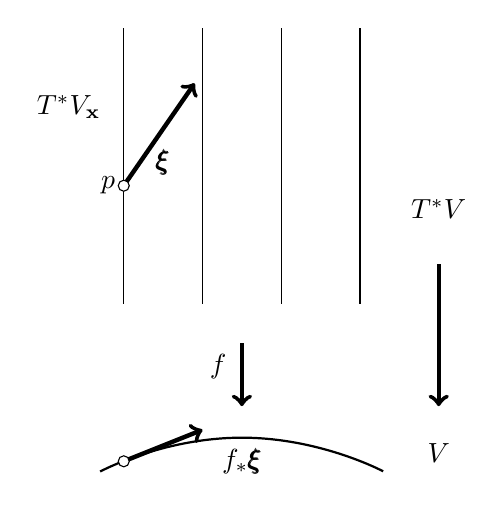
\begin{tikzpicture}
    % T^*V
    \draw [] (0, 2) -- (0, 5.5);
    \draw [] (1, 2) -- (1, 5.5);
    \draw [] (2, 2) -- (2, 5.5);
    \draw [] (3, 2) -- (3, 5.5);

    \node [] at (-0.7, 4.5) {$T^*V_{\mathbf x}$};

    % the mapping f
    \node [] at (1.2, 1.2) {$f$};
    \draw [ultra thick, ->] (1.5, 1.5) -- (1.5, 0.7);

    \node [] at (4.0, 3.2) {$T^*V$};
    \draw [ultra thick, ->] (4.0, 2.5) -- (4.0, 0.7);
    \node [] at (4.0, 0.1) {$V$};

    % vector xi
    \draw [ultra thick, ->] (0, 3.5) -- (0.9, 4.8);
    \node [] at (0.5, 3.8) {$\pmb\xi$};

    % point p
    \node [] at (-0.2, 3.5) {$p$};
    \draw [fill=white] (0, 3.5) circle (0.07);

    % V space

    \draw [thick] plot [smooth, tension=1]
      coordinates{(-0.3, -0.13) (1.5, 0.3) (3.3, -0.13)};
    \node [] at (1.5, 0) {$f_*\pmb\xi$};

    \draw [ultra thick, ->] (0, 0) -- (1.0, 0.4);
    \draw [fill=white] (0, 0) circle (0.07);

  \end{tikzpicture}
  \label{fig:1form_cotangent}
  \caption{The 1-form $\mathbf p \, d\mathbf q$ on
    the cotangent bundle}
\end{figure}


\end{proof}

\begin{rem*}
Consider a lagrangian mechanical system with configuration manifold $V$
and lagrangian function $L$.
It is easy to see that the lagrangian ``generalized velocity''
$\dot{\mathbf q}$ is a tangent vector to the configuration manifold $V$,
and the ``generalized momentum''
$\dot{\mathbf p} = \partial L/\partial \dot{\mathbf q}$
is a cotangent vector.
Therefore, the ``$\mathbf p, \mathbf q$'' phase space of the lagriangian
system is the cotangent bundle of the configuration manifold.
The theorem above shows that the phase space of a mechanical problem
has a natural symplectic manifold structure.
%Let $L = L(\mathbf q, \dot{\mathbf q})$  be a Lagrangian.
%%
%Then, $\dot{\mathbf q}$ is a tangent vector;
%%
%$\mathbf p = \partial L/\partial \dot{\mathbf q}$
%is a cotangent vector.
%%
%The $\mathbf p, \mathbf q$ phase space of the Lagrangian system
%is the cotangent of the configuration manifold.
%%
%The above theorem shows that the phase space of
%a mechanical problem has a natural symplectic
%manifold structure.
\end{rem*}

\begin{prob*}
  Show that the Legendre transform does not depend on the coordinate system:
  it takes a fucntion $:TV \rightarrow \mathbb R$ on the tangent bundle
  to a function $H: T^*V \rightarrow \mathbb R$ on the cotangent bundle.


\answer{
  Consider a coordinate transform $\mathbf q = \mathbf q(\mathbf Q)$,
  $$
  \begin{aligned}
  H
  &= \sum_i \dot q_i\frac{ \partial L } { \partial \dot q_i } - L
  = \sum_{ijk}
    \dot Q_j \frac{\partial q_i}{\partial Q_j}
    \frac{ \partial Q_k } { \partial q_i }
    \frac{ \partial L } { \partial Q_k } - L \\
  &= \sum_{jk}
    \dot Q_j \delta_{jk}
    \frac{ \partial L } { \partial Q_k } - L
  = \sum_j \dot Q_j \frac{ \partial L } { \partial Q_j } - L.
  \end{aligned}
  $$
  Thus the hamiltonian function is the same in the two coordinates.
}
\end{prob*}

% subsection C
\subsection{Hamiltonian vector fields}



A Riemann structure on a manifold establishes an isomorphism between
the spaces of tangent vectors and 1-forms.
%
A symplectic structure establishes a similar isomorphism.


\begin{defn*}
%
To each vector $\pmb \xi$
tangent to a symplectic manifold $(M^{2n}, \omega^2)$
at point $\mathbf x$, we associate a 1-form $\omega^1_{\pmb \xi}$
on $TM_{\mathbf x}$ by the formula
$$
\omega^1_{\pmb \xi}(\pmb \eta) = \omega^2(\pmb \eta, \pmb \xi),
\quad \forall \pmb \eta \in TM_{\mathbf x}.
$$
\end{defn*}

\begin{prob*}
Show that the correspondence $\pmb \xi \rightarrow \omega^1_{\mathbf \xi}$
is an isomorphism between the $2n$-dimensional vector spaces of vectors
and of 1-forms.
\end{prob*}

\begin{ex*}
  In $\mathbb{R}^{2n}=\{(\mathbf p, \mathbf q)\}$
  we will identify vectors and 1-forms by using the euclidean structure
  $(\mathbf x, \mathbf x) = \mathbf p^2 + \mathbf q^2$.
  Then the correspondences $\pmb\xi \rightarrow \omega^1_{\pmb\xi}$
  determines a transformation
  $\mathbb{R}^{2n} \rightarrow \mathbb{R}^{2n}$.
\end{ex*}

\begin{prob*}
  Calculate the matrix of this transformation in the basis
  $\mathbf p,\mathbf q$.

\answer{
For $n = 1$,
$\omega^2 = \pmb \eta \wedge \pmb \xi = \eta_1 \xi_2 - \eta_2 \xi_1$.
Then
$\omega^1_{\pmb \xi}(\pmb \eta) = (\pmb \eta, \mathbf J^{-1} \pmb \xi)$,
where $\mathbf J^{-1}$ means a rotation of $-\pi/2$, where
$$
\mathbf J =
\left(
  \begin{array}{cc}
    0  & -1 \\
    1  & 0
  \end{array}
\right)
\qquad
\mathbf J^{-1} =
\left(
  \begin{array}{cc}
    0  & 1 \\
    -1 & 0
  \end{array}
\right),
$$
with the indices of $p$ and $q$ being $1$ and $2$, respectively
(the convention of this book).

For higher dimensions, we just replace $1$ by the $n\times n$
identity matrix $E$,
$$
\mathbf J =
\left(
  \begin{array}{cc}
    0  & -E \\
    E  & 0
  \end{array}
\right)
\qquad
\mathbf J^{-1} =
\left(
  \begin{array}{cc}
    0  & E \\
    -E & 0
  \end{array}
\right).
$$
}

\note{
  \label{note:J_R2n}
Generally, we have
$$
\omega^1_{\pmb \xi}(\pmb \eta) = (\pmb \eta, \mathbf I^{-1} \pmb \xi)
=\eta' \mathbf J^{-1} \pmb\xi.
$$
with the prime``$'$'' denoting the transpose.

However, later in this book, the author will frequently use the result
$$
\omega^2(\pmb\eta,\pmb\xi) = (I\pmb\eta, \pmb\xi) = \pmb\eta'\mathbf J' \pmb\xi,
$$
for this case. This is not generally true.
It requires the isomorphism $I$ to be equivalent to a matrix multiplication
of the symplectic matrix $\mathbf J$, and $\mathbf J' = \mathbf J^{-1}$.

In general,
$\omega^1_{\pmb \xi}$ is represented by the vector $I^{-1} \pmb \xi$,
and a 1-form $\omega_1$ is represented by the vector $I\, \omega_1$.
}
\end{prob*}
%






We will denote by $I$ the isomorphism
$I: T^*M_{\mathbf x} \rightarrow TM_{\mathbf x}$
(from 1-forms to tangent vectors,
$\omega^1_{\pmb \xi} \rightarrow \pmb \xi$).
%
Now let $H$ be a function on a symplectic manifold $M^{2n}$.
%
Then $dH$ is a differential 1-form on $M$ and
for every point there is a tangent vector to $M$ associated to it.
%
In this way, we obtain a vector field $IdH$ on $M$.


\begin{defn*}
%
The vector field $IdH$ is called \emph{hamiltonian vector field}.
%
$H$ is called the \emph{hamiltonian function}.
\end{defn*}

\begin{ex*}
  If $M^{2n} = R^{2n} = {(\mathbf p, \mathbf q)}$,
  then we obtain the phase velocity field
  of Hamilton's canonical equation:
  $$
  \dot{\mathbf x} = I\,dH(\mathbf x)
  \Longleftrightarrow
  \dot{\mathbf p} = - \frac{\partial H }{ \partial \mathbf q}
  \mathrm{\quad and \quad}
  \dot{\mathbf q} = \frac{\partial H}{\partial \mathbf p}.
  $$
\note{In the above example,
the 1-form is represented by the vector
$\nabla H = \left(\frac{\partial H}{\partial \mathbf p},
\frac{\partial H}{\partial q}\right)^T$
to invert this vector to corresponding tangent vector we multiple it by $\mathbf J$
%
\[
\arraycolsep=3.0pt\def\arraystretch{1.5}
\mathbf J \cdot \nabla H
=
\left(
  \begin{array}{ccc}
    0 & -1 \\
    1 & 0
  \end{array}
\right)
\left(
  \begin{array}{ccc}
    \frac{ \partial H }{ \partial \mathbf p } \\
    \frac{ \partial H }{ \partial \mathbf q }
  \end{array}
\right)
=
\left(
  \begin{array}{ccc}
    -\frac{ \partial H }{ \partial \mathbf q } \\
    \frac{ \partial H }{ \partial \mathbf p }
  \end{array}
\right)
=
\left(
  \begin{array}{ccc}
    \dot{\mathbf p} \\
    \dot{\mathbf q}
  \end{array}
\right).
\]}
\end{ex*}




\summary{
  \begin{enumerate}
    \item
      A $2n$-dimensional differentiable manifold, $M^{2n}$,
      along with a \emph{closed nondegenerate} 2-form $\omega^2$,
      is called a \emph{symplectic manifold}.
      The 2-form is called the \emph{symplectic structure}.
      Usually, the manifold has $n$ momentum components
      and $n$ coordinate components,
      and the 2-form is $\omega^2 = \sum_{i = 1}^n dp_i \wedge dq_i$.

    \item
      We can construct a $2n$-dimensional symplectic manifold
      from an $n$-dimensional differentiable manifold $V$.
      %
      At each point $\mathbf x \in V$, the 1-forms, written as
      $\omega^1 = \sum_{i=1}^n p_i dq_i$ in local coordinates,
      span an $n$-dimensional vector space for the coefficients
      $(p_1, \dots, p_n)$.
      This vector space is the \emph{cotangent space} $T^*V_\mathbf{x}$.
      %
      By supplementing each point $\mathbf x$
      by the cotangent space $T^V_\mathbf{x}$,
      we get a $2n$-dimensional joint space of
      $\mathbf x$ (with local coordinates $q_1, \dots, q_n$,
      and 1-forms $p_1, \dots, p_n$),
      called the \emph{cotangent bundle} $T^*V$.
      %
      Then we get a symplectic manifold $(T^*V, \omega^2)$,
      with $\omega^2 = \sum_i dp_i \wedge dq_i = d\left(\sum_i p_i dq_i \right)$.

    \item
      In the symplectic space,
      there is an isomorphism $I$ between 1-forms $\omega^1$
      and tangent vector, $\pmb\xi = I\omega^1$
      through the 2-form of the symplectic structure
      $$
      \omega^1_{\pmb\xi}(\pmb\eta)
      =
      \omega^2(\pmb\xi, \pmb\eta).
      $$
      In local coordinates of the euclidean space,
      $I$ is equivalent to multiplying symplectic matrix
      $$
      \mathbf J =
      \left(
        \begin{array}{ccc}
          0 & -E \\
          E & 0
        \end{array}
      \right)
      $$
      to a vector corresponding to the 1-form,
      e.g., $\nabla H = (\partial H/\partial \mathbf p, \partial H/\partial \mathbf q)$.

  \end{enumerate}
}





%section 38
\section{Hamiltonian phase flows and their integral invariants}

Liouville's theorem asserts that the phase flow
preserve the symplectic structure.
%
Poincar\'e found a whole series of differential forms
which are preserved by the hamiltonian flow.

%\subsection 38A
\subsection{Hamiltonian phase flows preserve the symplectic structure}

Let $(M^{2n}, \omega^2)$ be a symplectic manifold and
$H: M^{2n} \rightarrow \mathbb{R}$ a function.
Assume that the vector field $IdH$
corresponds to $H$ gives a 1-parameter group
of diffeomorphism: $g^t: M^{2n} \rightarrow M^{2n}$:
$$
\left.\frac{d}{dt}\right|_{t = 0} g^t\mathbf x
= I dH(\mathbf x).
$$
This group $g^t$ is the hamiltonian phase flow with
hamiltonian function $H$.

\note{
A \emph{diffeomorphism} is an isomorphism of smooth manifolds.
It is a smooth invertible function that maps one differentiable manifold
to another.

Not all differentiable maps are diffeomorphism, because of the one-to-one requirement.
For example, $(x, y) \rightarrow (y^2 \sin x, y^2 \cos x)$ is not invertible.
}

\begin{thm}
A hamiltonian phase flow preserves the symplectic structure:
$$
(g^t)^* \omega^2 = \omega^2.
$$
\end{thm}

\note{The difference between $g^t$ and $(g^t)^*$:
  $g^t$ applies to a point $\mathbf x$ or a tangent vector on the manifold $M$,
  $(g^t)^*$ applies to a differential form $\omega$.
  The definition of
  $$
  \left[ (g^t)^*\omega^2_{\mathbf x} \right](\pmb\xi, \pmb\eta)
  \equiv
  \omega^2_{g^t \mathbf x}(g^t\pmb\xi, g^t\pmb\eta).
  $$
  Here $\omega^2_{\mathbf x}$ means the 2-form evaluated at $\mathbf x$.
  See details in Sec. 33C.
  Generally, a 2-form depends on not only the tangent vectors,
    $\pmb\xi$ and $\pmb\eta$,
    but also the point $\mathbf x$ on the manifold.
  But for $\omega^2 = d\mathbf p \wedge \mathbf q$,
    this dependence is missing.
  In this book, the subscript is often omitted.
  We shall sometimes add it back in the notes for clarity.
}


In the case $n = 1$, $M^{2n} = \mathbb{R}^2$, this theorem says
that the phase flow $g^t$ preserves area (Liouville's theorem).

For the proof of this theorem, it is useful to introduce
the following notation.

Let $M$ be an arbitrary manifold,
$c$ a $k$-chain on $M$ and $g^t: M \rightarrow M$
a one-parameter family of differentiable mappings.
We will construct a $(k+1)$-chain $Jc$ on $M$,
which we will call the
\emph{track of the chain $c$ under the homotopy
$g^t$, $0 \le t \le \tau$}.
\note{Roughly, ``homotopy'' means time evolution.}


Let $(D, f, \mathrm{Or})$ be one of the cells in the chain $c$.
\note{$D$ is the domain, a convex polygon in $\mathbb{R}^k$,
  $f$ is a mapping from the euclidean space to the manifold $\mathbb{R}^k \rightarrow M$,
  $\mathrm{Or}$ is the orientation.
  See page 184, \S 35.D.}
%
To this cell will be associated a cell $(D', f', \mathrm{Or}')$
  in the chain $Jc$ where $D' = I\times D$ is the direct product
  of the interval of $0 \le t \le \tau$ and $D$;
  the mapping $f': D' \rightarrow M$ is obtained from
  $f: D \rightarrow M$ by the formula
  $f'(t, x) = g^t f(x)$;
  and the orientation $\mathrm{Or}'$ of the space $\mathbb{R}^{k+1}$
  containing $D'$ is given by the frame
  $\mathbf e_0, \mathbf e_1, \dots, \mathbf e_k$,
  where $\mathbf e_0$ is the unit vector of the $t$ axis,
  and $\mathbf e_1, \dots, \mathbf e_k$ is an oriented frame for $D$.


We could say that $Jc$ is the chain swept out by $c$
  under the homotopy $g^t$, $0 \le t \le \tau$.
  The boundary of the chain $Jc$ consists of ``end-walls''
  made up of the initial and final positions of $c$,
  and the ``side surfaces'' filled in by the boundary of $c$.
\note{Below, we want to prove that the integrals on the side surfaces
  vanishes, so is the integral on the volume enclosed by the tube.
  Then the integrals at the two end walls, which are opposite
  in the signs must add to zero.}

\setcounter{figure}{166}
\begin{figure}
\centering
  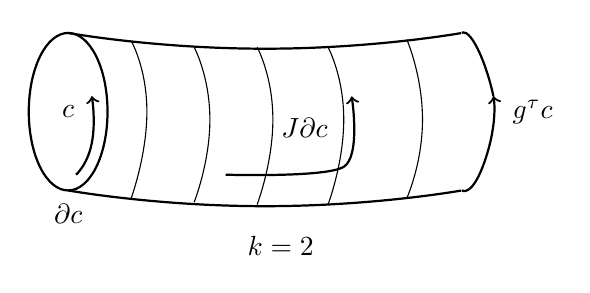
\begin{tikzpicture}
    % end-wall 1
    \draw [thick] plot [smooth cycle, tension=1]
      coordinates{(0, 0) (0.5, 1) (0, 2) (-0.5, 1)};
    % bottom of side surface
    \draw [thick] plot [smooth, tension=1]
      coordinates{(0, 0) (2.5, -0.2) (5, 0)};
    % top of the side surface
    \draw [thick] plot [smooth, tension=1]
      coordinates{(0, 2) (2.5,  1.8) (5, 2)};
    % end-wall 2
    \draw [thick, ->] plot [smooth, tension=1.5]
      coordinates{(5, 0) (5.3, 0.4) (5.4, 1.2)};
    \draw [thick] plot [smooth, tension=1.2]
    coordinates{(5.4, 1.2) (5.2, 1.8) (5, 2)};

    % intermediate rings
    \draw [] plot [smooth, tension=1]
      coordinates{(0.8, -0.1) (1.0, 1.0) (0.8, 1.9)};
    \draw [] plot [smooth, tension=1]
      coordinates{(1.6, -0.15) (1.8, 0.9) (1.6, 1.82)};
    \draw [] plot [smooth, tension=1]
      coordinates{(2.4, -0.18) (2.6, 0.9) (2.4, 1.82)};
    \draw [] plot [smooth, tension=1]
      coordinates{(3.3, -0.18) (3.5, 0.9) (3.3, 1.82)};
    \draw [] plot [smooth, tension=1]
      coordinates{(4.3, -0.1) (4.5, 0.9) (4.3, 1.92)};

    % dc
    \draw [->, thick] plot [smooth, tension=1]
      coordinates{(0.1, 0.2) (0.3, 0.6) (0.3, 1.2)};
    \node[](dc) at (0, -0.3){$\partial c$};

    % c
    \node[](c) at (0, 1.0){$c$};

    % J dc
    \draw [->, thick] plot [smooth, tension=0.5]
      coordinates{(2, 0.2) (3.5, 0.3) (3.6, 1.2)};
    \node[](Jc) at (3, 0.8){$J\partial c$};

    % g c
    \node[](gc) at (5.9, 1.0){$g^\tau c$};

    % k = 2
    \node[](keq2) at (2.7, -0.7){$k = 2$};
  \end{tikzpicture}
%
  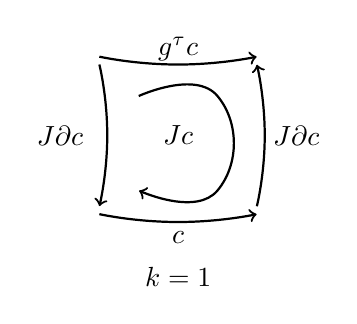
\begin{tikzpicture}
    % c
    \draw [thick, ->] plot [smooth, tension=1]
      coordinates{(0, 0) (1, -0.1) (2, 0)};
    \node[](c) at (1, -0.3){$c$};
    % g c
    \draw [thick, ->] plot [smooth, tension=1]
      coordinates{(0, 2) (1., 1.9) (2, 2)};
    \node[](gc) at (1, 2.1){$g^\tau c$};
    % J c, left
    \draw [thick, ->] plot [smooth, tension=1]
      coordinates{(0, 1.9) (0.1, 1) (0, 0.1)};
    \node[](Jcleft) at (-0.5, 1){$J\partial c$};
    % J c, right
    \draw [thick, ->] plot [smooth, tension=1]
      coordinates{(2, 0.1) (2.1, 1) (2, 1.9)};
    \node[](Jcright) at (2.5, 1){$J\partial c$};

    % the circle
    \draw [thick, ->] plot [smooth, tension=1.0]
      coordinates{(0.5, 1.5) (1.5, 1.5) (1.5, 0.3) (0.5, 0.3)};
    \node[](Jc) at (1, 1){$Jc$};
    % k = 1
    \node[](gc) at (1.0, -0.8){$k = 1$};
  \end{tikzpicture}
  \caption{Track of a cycle under homotopy. \\
    %
    \note{ On the sign of the terms in \eqref{eq:c_homotopy}.\\
      %
      For $k = 2$ (left panel),
      $c$ represents an oriented area,
      which is positive for $-\mathbf x = \mathbf z \times \mathbf y$ direction;
      so the boundary $\partial c$ is positive
      for a counterclockwise rotation around the axis $-\mathbf x$.
      %
      The positive direction of $J$ represents a vector along $+\mathbf x$.
      %
      Thus for a correctly oriented volume element $Jc$,
      its sign should be negative, as
      $(\mathbf x, \mathbf z, \mathbf y) = \mathbf x \cdot (\mathbf z \times \mathbf y) < 0$.
      %
      $\partial (Jc)$, pointing to a direction of increasing $Jc$,
      or equivalently decreasing the absolute volume,
      is positive along the direction into the volume.
      %
      $J \partial c$ representing an oriented area element,
      is positive for the counterclockwise direction
      on the face facing the reader, as indicated by the arrow in the figure.
      %
      This means $J \partial c$ points out of the side surfaces,
      opposite to the direction of $\partial (Jc)$.
      %
      Since the positive direction of $c$ ($-\mathbf x$) is pointing out of the volume,
      it is opposite to the sign of $\partial (Jc)$.
      %
      Since the positive direction of $g^\tau c$ ($-\mathbf x$) is pointing into the volume,
      it shares the same sign as $\partial (Jc)$.
      %
      \\
      %
      For $k = 1$ (right panel),
      $c$ is an oriented line element
      which is positive along the $+\mathbf x$ direction.
      %
      The boundary $\partial c$ is the difference between the two points,
      positive for the final (larger $x$) point,
      and negative for the initial (smaller $x$) point.
      %
      The direction of $J$ is along the $+\mathbf y$ axis.
      %
      Thus, the positive direction of $Jc$ should be along
      $\mathbf y \times \mathbf x$
      ($c$ for $+\mathbf x$),
      a direction pointing into the paper.
      %
      It follows that the direction of $\partial(Jc)$ should be clockwise,
      according to the right-hand rule.
      %
      In this case, $J\partial c$ is $J$ multiplied by the sign of $\partial c$
      Thus, $J \partial c$ is positive for the right edge,
      and negative for the left edge (this is why $J\partial c$
      goes downwards there).
      %
      Clearly, $J\partial c$ and $\partial (Jc)$ run in the opposite directions;
      %
      $c$ and $\partial (Jc)$ also run in the opposite directions;
      but
      $g^\tau c$ and $\partial (Jc)$ run int the same direction.
    }
  }
\end{figure}

It is easy to verify that under the choice of orientation made above
\begin{equation}
\partial (J c_k) = g^\tau c_k - c_k - J \partial c_k.
\label{eq:c_homotopy}
\end{equation}

\begin{lem*}
  Let $\gamma$ be a 1-chain in the symplectic manifold $(M^{2n}, \omega^2)$.
  Let $g^t$ be phase flow on $M$ with hamiltonian function $H$.
  Then
  $$
  \frac{d}{d\tau} \int_{J\gamma} \omega^2
  =
  \int_{g^\tau\gamma} dH.
  $$
\end{lem*}

\begin{proof}
  It is sufficient to consider a chain $\gamma$ with one cell
  $f: [0,1] \rightarrow M$.
  \note{$\gamma$ is a curve, which will be $\partial c$.}
  We introduce the notation
  $$
    f'(s, t) = g^t f(s),
    \qquad
    \pmb\xi = \frac{ \partial f' } { \partial s },
    \mathrm{\quad and \quad}
    \pmb\eta = \frac{ \partial f' } { \partial t }
    = TM_{f'(s, t)}.
  $$
  By the definition of the integral,
  $$
  \int_{J\gamma} \omega^2
  =
  \int_0^1 \int_0^\tau \omega^2(\pmb\xi, \pmb\eta) \, dt \, ds.
  $$
  \note{There might be a missing minus sign:
    $\int_{J\gamma} \omega^2$ should really mean
    $\int_0^\tau \int_0^1 \omega^2(\pmb\eta, \pmb\xi) \, dt \, ds$,
    for, by literal translation, $J$ goes before $\gamma$,
    hence $\pmb\eta$ before $\pmb\xi$.
    This doesn't cause trouble, because we only consider
    closed chains (see the next Corollary).
    For closed chains, the integral vanishes, and
    the sign doesn't matter.
  }
  But by the definition of the phase flow,
  $\pmb \eta$ is a vector (at the point $f'(s, t)$)
  of the hamiltonian flow with hamiltonian function $H$.
  \note{$\pmb\eta = I dH$.}
  By defintion of a hamiltonian field
  $\omega^2(\pmb\xi, \pmb\eta) = dH(\pmb\xi)$.
  \begin{figure*}
    \centering
    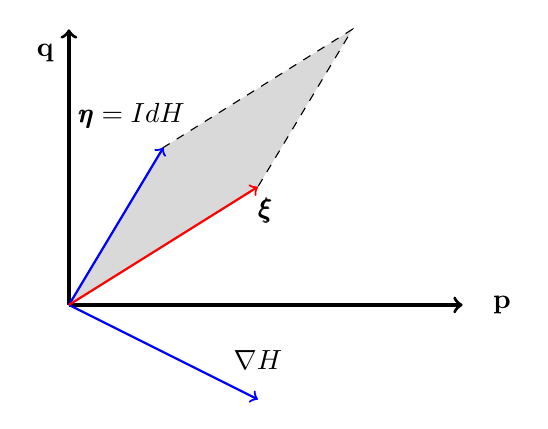
\begin{tikzpicture}
      % q axis
      \draw [very thick, ->] (0,0) -- (0,3.5);
      \node[](q) at (-0.3, 3.2){$\mathbf q$};

      % p axis
      \draw [very thick, ->] (0,0) -- (5,0);
      \node[](p) at (5.5, 0){$\mathbf p$};

      % the parallelogram
      \draw [dashed, fill=gray!30!white] (0, 0) -- (1.2, 2) -- (3.6, 3.5) -- (2.4, 1.5) -- cycle;

      % dH
      \draw [thick, ->, blue] (0, 0) -- (2.4, -1.2);
      \node[](dH) at (2.4, -0.7){$\nabla H$};

      % eta = IdH
      \draw [thick, ->, blue] (0, 0) -- (1.2, 2);
      \node[](IdH) at (0.8, 2.4){$\pmb\eta = I dH$};

      % xi
      \draw [thick, ->, red] (0, 0) -- (2.4, 1.5);
      \node[](eta) at (2.5, 1.2){$\pmb\xi$};
    \end{tikzpicture}
    \caption*{Illustration of $\omega^2(\pmb\xi, \pmb\eta) = (\pmb\xi, \nabla H)$.
    The area spanned by $\pmb\xi$ and $\pmb\eta = IdH$ is equal
    to the projection of $\nabla H$ on $\pmb \xi$.}
  \end{figure*}
    \note{$\omega^2(\pmb\xi, \pmb\eta) = \omega^1_{\pmb\eta}(\pmb\xi)
      = \omega^1_{IdH}(\pmb\xi) = (\pmb\xi, I^{-1} IdH)
    = dH(\pmb\xi)$.}
  Thus,
  $$
  \int_{J\gamma}\omega^2 = \int_0^\tau
  \left(
    \int_{g^t\tau} dH
  \right) dt.
  $$
  \note{
    $\int_0^1 \omega^2(\pmb\xi, \pmb\eta) \, ds
    = \int_0^1 dH(\pmb\xi) \, ds = \int_0^1 dH(\pmb\xi \, ds).$
    But $\pmb\xi = \frac{ \partial f' } { \partial s }
    = g^t \frac{ d f }{ d s } \rightarrow
    \pmb\xi\, ds = g^t \, df = d(g^t f)$,
    So
    $\int_0^1 dH(\pmb\xi ds) = \int dH(d g^t f) = \int_{g^t\gamma} dH.$
  }
\end{proof}


\begin{cor*}
  If the chain $\gamma$ is closed ($\partial \gamma = 0$)
  then $\int_{J\gamma} \omega^2 = 0$.
\end{cor*}

\begin{proof}
  $\int_\gamma dH = \int_{\partial \gamma} H = 0.$

  \note{
    $-\int_{J\gamma} \omega^2 = \int_0^\tau \int_{g^t\gamma} dH \, dt
    = \int_0^\tau dt \int_{\partial(g^t \gamma)} H
    = \int_0^\tau dt \int_{g^t\partial\gamma} H = 0.$
  }
\end{proof}

\begin{proof}[Proof of the theorem.]
  We consider any 2-chain $c$. We have
  $$
  0 \stackrel{1}{=} \int_{Jc} d\omega^2
  \stackrel{2}{=} \int_{\partial Jc} \omega^2
  \stackrel{3}{=}
  \left(
    \int_{g^\tau c}
    -\int_{c}
    -\int_{J\partial c}
  \right)
  \omega^2
  \stackrel{4}{=}
  \left(
    \int_{g^\tau c}
    -\int_{c}
  \right)
  \omega^2.
  $$
  (1 since $\omega^2$ is closed, 2 by Stokes formula,
  3 by formula \eqref{eq:c_homotopy},
  4 by the corollary above with $\gamma = \partial c$).
  Thus the integrals of the form $\omega^2$
  on any chain $c$ and on its image $g^\tau c$ are the same.
\end{proof}


% subsection B
\subsection{Integral invariants}

Let $g:M\rightarrow M$ be a differentiable map.

\begin{defn*}
  A differential $k$-form $\omega$ is called an \emph{integral invariant}
  of the map $g$ if the integrals of $\omega$ on
  any $k$-chain $c$ and on its image under $g$ are the same:
  \begin{equation}
  \int_{gc}\omega = \int_c \omega.
  \label{eq:integral_invariant}
  \end{equation}
\end{defn*}

\note{The precise meaning of \eqref{eq:integral_invariant} is the following.
  Let $f$ be a mapping from $\mathbb R$ to $M$,
  For a $k$-chain $c$ with one cell:
  $f:[0, 1]^k \rightarrow M$,
  we have $f(\mathbf s) \in M$ for $\mathbf s \in [0,1]^k$.
  %
  The $k$ tangent vectors are defined as
  $\pmb\xi_i = \partial f/\partial s_i$
  for $i = 1, \dots k$.
  %
  Then, for a $k$-form $\omega = \omega^k$,
  the right-hand side reads
  $$
  \int_{c} \omega
  =
  \int_0^1 \dots \int_0^1
    \omega^k_{f \mathbf s}(\pmb\xi_1,\dots, \pmb\xi_k)
    \, ds_1 \cdots ds_k
  =
  \int_0^1 \dots \int_0^1
    \omega^k_{\mathbf x}(\pmb\xi_1,\dots, \pmb\xi_k)
    \, ds_1 \cdots ds_k.
  $$
  The left-hand side reads
  $$
  \int_{gc} \omega
  =
  \int_0^1 \dots \int_0^1
    \omega^k_{(g \circ f)\, \mathbf s}(g \pmb\xi_1,\dots, g \pmb\xi_k)
    \, ds_1 \cdots ds_k
  =
  \int_0^1 \dots \int_0^1
    \omega^k_{g \mathbf x}(g \pmb\xi_1,\dots, g \pmb\xi_k)
    \, ds_1 \cdots ds_k.
  $$
  The point to note here is that \eqref{eq:integral_invariant}
  implicitly assumes the transformation $g$ on the coordinates $\mathbf x$
  and the tangent vectors $\pmb\xi_1, \dots, \pmb\xi_k$,
  on the left-hand side.
}

\begin{ex*}
  If $M = \mathbb{R}^2$ and $\omega^2 = dp \wedge dq$ is the area element,
  then $\omega^2$ is an integral invariant of any map $g$
  with jacobian $1$.
\end{ex*}

\begin{prob*}
  Show that a form $\omega^k$ is an integral invariant
  of a mapping if and only if $g^*\omega^k = \omega^k$.

  \answer{
    It is sufficient to consider a chain $c$ with one cell
    $f: [0, 1]^k \rightarrow M$.
    Then using the above notation,
    for $\mathbf x = f\mathbf s \in M$, and
    $\xi_i = \partial f/\partial s_i$,
    we have
    $$
    \begin{aligned}
      \int_{gc} \omega^k
      &=
      \int_0^1 \dots \int_0^1 \omega^k_{g\mathbf x}
      (g\pmb\xi_1, \dots, g\pmb\xi_k)
          \,ds_1 \dots ds_k
      \\
      &=
      \int_0^1 \dots \int_0^1 \left( g^*\omega^k_{\mathbf x} \right)
      (\pmb\xi_1, \dots, \pmb\xi_k)
          \,ds_1 \dots ds_k
      =
      \int_c g^*\omega^k.
    \end{aligned}
    $$
    Note that $\omega^k$ on the left is integrated over $gc$,
    $g^*\omega^k$ on the right over $c$.
    Conceptually, $gc$ and $c$ can be thought as chains
    of two different manifolds $gM$ and $M$.

    If $g^*\omega^k = \omega^k$, then
    $\int_{gc} \omega^k = \int_c \omega^k$,
    and $\omega^k$ is an integral invariant of $g$.

    Conversely, if $\omega^k$ is an integral invariant,
    then
    $\int_{c} \omega^k = \int_{gc} \omega^k = \int_c g^*\omega^k$,
    for any $k$-chain $c$, so
    $g^*\omega^k = \omega^k$.

    While this result follows straightforwardly from definition,
    it expresses two different ways of thinking
    of integral invariants.
    First,
    $\int_{gc}\omega = \int_c \omega$
    means that we get the same number from integrating
    the chains before and after the mapping $g$.
    %
    Alternatively,
    $g^* \omega = \omega$ means that if we stick
    to the chain before the mapping but
    inversely transform the form $\omega$ by $g^*$,
    we get the same result after integration.
  }
\end{prob*}

\begin{prob*}
  Show that if the forms $\omega^k$ and $\omega^l$
  are integral invariants of the map,
  then the form $\omega^k \wedge \omega^l$
  is also an integral invariant of $g$.

  \answer{
    It follows from Problem \ref{prob:fstar_exprod} in Sec. 33.
    $$
    \begin{aligned}
    \int_{gc} (\omega^k \wedge \omega^l)
    &=
    \int_{c} (\omega^k \wedge \omega^l)(g\pmb\xi_1, \dots, g\pmb\xi_{k+l})
    =
    \int_{c} g^*(\omega^k \wedge \omega^l)(\pmb\xi_1, \dots, \pmb\xi_{k+l})
    \\
    &=\int_{c} (g^*\omega^k \wedge g^*\omega^l)(\pmb\xi_1, \dots, \pmb\xi_{k+l})
    =\int_{c} (\omega^k \wedge \omega^l)(\pmb\xi_1, \dots, \pmb\xi_{k+l}).
    \end{aligned}
    $$
  }
\end{prob*}

The theorem in subsection A can be reformulated as follows.

\begin{thm*}
  The form $\omega^2$ giving the symplectic structure
  is an integral invariant of a hamiltonian phase flow.
\end{thm*}

We now consider the exterior powers of $\omega^2$,
$$
(\omega^2)^2 = \omega^2 \wedge \omega^2,
\quad
(\omega^2)^3 = \omega^2 \wedge \omega^2 \wedge \omega^2,
\dots
$$

\begin{cor*}
  Each of the forms $(\omega^2)^2$, $(\omega^2)^3$, $(\omega^2)^4$, \dots
  is an integral invariant of a hamiltonian phase flow.
\end{cor*}

\begin{prob*}
Suppose that the dimension of the symplectic manifold
$(M^{2n}, \omega^2)$ is $2n$,
show that $(\omega^2)^k = 0$ for $k > n$,
and that $(\omega^2)^n$ is a nondegenerate $2n$-form on $M^{2n}$.
\end{prob*}

We define a volume element on $M^{2n}$ using $(\omega^2)^n$.
Then, a hamiltonian phase flow preserves volume,
and we obtain Liouville's theorem from the corollary above.

\begin{ex*}
  Consider the symplectic coordinate space
  $M^{2n} = \mathbb R^{2n} = \{(\mathbf p, \mathbf q)\}$,
  $\omega^2 = d\mathbf p \wedge d\mathbf q = \sum dp_i \wedge dq_i$.
  In this case the form $(\omega^2)^k$ is proportional to the form
  $$
  \omega^{2k} = \sum_{i_1 < \dots < i_k}
  dp_{i_1} \wedge \dots \wedge dp_{i_k} \wedge
  dq_{i_1} \wedge \dots \wedge dq_{i_k}.
  $$
  The integral of $\omega^{2k}$ is equal to the sum of
  the oriented volumes of projections on to the coordinate planes
  $(p_{i_1}, \dots, p_{i_k}, q_{i_1}, \dots, q_{i_k})$.
\end{ex*}

The map
$g: \mathbb R^{2n} \rightarrow \mathbb R^{2n}$
is called \emph{canonical} if it has $\omega^2$ as an integral invariant.
A canonical map is generally called a \emph{canonical transformation}.
Each of the forms $\omega^4, \omega^6, \dots, \omega^{2n}$
is an integral invariant of every canonical transformation.
Therefore, \emph{under a canonical transformation,
  the sum of the oriented areas of projections onto the coordinate planes
  $(p_{i_1}, \dots, p_{i_k}, q_{i_1}, \dots, q_{i_k})$,
  $1 \le k \le n$, is preserved}.
In particular, \emph{canonical transformations preserve volume}.

The hamiltonian phase flow given by the equations
$\dot{\mathbf p} = -\partial H/\partial \mathbf q$,
$\dot{\mathbf q} = \partial H/\partial \mathbf p$
consists of canonical transformations $g^t$.

The integral invariants considered above are also called
\emph{absolute integral invariants}.

\begin{defn*}
  A differential $k$-form is called a
  \emph{relative integral invariant} of the map
  $g: M \rightarrow M$ if
  $\int_{gc} \omega = \int_c \omega$
  for every \emph{closed} $k$-chain $c$.
\end{defn*}

\begin{thm*}
  Let $\omega$ be a relative integral invariant of a map $g$.
  Then $d\omega$ is an absolute integral invariant of $g$.
\end{thm*}

\begin{proof}
  Let $c$ be a $k+1$-chain. Then
  $$
  \int_c d\omega \stackrel{1}{=}
  \int_{\partial c} \omega
  \stackrel{2}{=}
  \int_{g\partial c} \omega
  \stackrel{3}{=}
  \int_{\partial gc} \omega
  \stackrel{4}{=}
  \int_{gc} d\omega.
  $$
  (1 and 4 are by Stokes' formula,
  2 by the definition of relative invariant,
  and 3 by the definition of boundary).
\end{proof}


\begin{ex*}
  A canonical map $g:\mathbb R^{2n} \rightarrow \mathbb R^{2n}$
  has the 1-form
  $$
  \omega^1 = \mathbf p \, d\mathbf q = \sum_{i = 1}^n p_i \, dq_i
  \mbox{ as a relative integral invariant.}
  $$
  \note{This is more like a converse of the above theorem,
  not a deduction.}
  In fact, every closed chain $c$ on $\mathbb R^{2n}$
  is the boundary of some chain $\sigma$
  \note{Recall the cone construction in Sec. 36},
  and we find
  $$
  \int_{gc} \omega^1
  \stackrel{1}{=}
  \int_{g\partial \sigma} \omega^1
  \stackrel{2}{=}
  \int_{\partial g\sigma} \omega^1
  \stackrel{3}{=}
  \int_{g\sigma} d\omega^1
  \stackrel{4}{=}
  \int_{\sigma} d\omega^1
  \stackrel{5}{=}
  \int_{\partial \sigma} \omega^1
  \stackrel{6}{=}
  \int_{c} \omega^1.
  $$
  (1 and 6 are by definition of $\sigma$,
  2 by definition of $\partial$,
  3 and 5 by Stokes' formula,
  and 4 since $g$ is canonical and
  $d\omega^1 = d(pdq) = dp \wedge dq = \omega^2$).
\end{ex*}


\begin{prob*}
  Let $d\omega^k$ be an absolute integral invariant of the map
  $g: M \rightarrow M$. Does it follow that $\omega^k$ is a
  relative integral invariant?
\end{prob*}

\begin{ans*}
  No, if there is a closed $k$-chain on $M$ which is not a boundary.
  \note{
  We still have
  $
  \int_{g\partial c} \omega^k =
  \int_{gc} d\omega^k =
  \int_c d\omega^k =
  \int_{\partial c} \omega^k.
  $
  The problem is that there are closed chains $\gamma$ that cannot be
  written as $\partial c$, like an equator of the torus, $T^2$,
  which will fail $\omega^k$.
  }
\end{ans*}


% subsection C
\subsection{The law of conservation of energy}

\begin{thm*}
  The function $H$ is a first integral of the hamiltonian phase flow
  with hamiltonian function $H$.
\end{thm*}

\begin{proof}
  The derivative of $H$ in the direction of a vector $\pmb\eta$
  is equal to the value of $dH$ on $\pmb\eta$.
  By definition of the hamiltonian field
  $\pmb\eta = IdH$ we find
  $$
  dH(\pmb\eta) = \omega^2(\pmb\eta, IdH)
  = \omega^2(\pmb\eta, \pmb\eta) = 0.
  $$
\end{proof}

\begin{prob*}
  Show that the 1-form $dH$ is an integral invariant
  of the phase flow with hamiltonian function $H$.

\answer{
  $$
  \left( \int_{g\gamma} - \int_{\gamma} \right) dH
  =
  \int_{\partial(Jc) } dH + \int_{J\partial c} dH
  =
  \int_{Jc} ddH + \int_0^1 dH(\pmb\eta) \, dt
  = 0 + 0 = 0.
  $$
}
\end{prob*}



\summary{
  \begin{enumerate}
    \item \emph{A hamiltonian phase flow preserves the symplectic structure.}
      $\int \omega^2_{g\mathbf x}(g^t\pmb\xi, g\pmb\eta)
      = \int \omega^2_{\mathbf x}(\pmb\xi, \pmb\eta)$,
      which means the integral of $\omega^2$ over any chain $c$
      gives the same value as the integral of $\omega^2$
      over the time evolved chain $g^t c$.

    \item The result is shown using the homotopy formula
      by constucting a tube of phase flow connecting the two chains
      $c$ and $g^tc$.

    \item Generally, if a form $\omega$ is invariant under a differentiable map $g$
      $\int_{gc} \omega = \int_c \omega$ is called an \emph{integral invariant} of $g$.

    \item If two forms $\omega^k$ and $\omega^l$ are integral invariants of $g$,
      so is their exterior product $\omega^k \wedge \omega^l$.

    \item So $\omega^2$ of the symplectic structure is an integral invariant
      of \emph{any} phase flow, so are the powers of
      $(\omega^2)^2, \dots, (\omega^2)^n$.

    \item A \emph{relative integral invariant} is a less restrict concept
      than the above \emph{absolute} integral invariant.
      It requires $\int_{gc} \omega = \int_c \omega$
      only for closed $c$-chains.

    \item If $\omega$ is a relative integral invariant,
      then $d\omega$ is an absolute integral invariant.
      However, the converse is not always true
      (although true for vector space):
      if $d\omega$ is an aboslute integral invariant,
      $\omega$ is not necessarily a relative integral invariant
      ($\omega$ is invariant for boundaries $\partial c$,
      but not all closed chains are not boundaries,
      e.g., when $M$ is a torus).

    \item The hamiltonian function $H$ is conserved
      along the phase flow $IdH$.
  \end{enumerate}
}



% section 39
\section{The Lie algebra of vector fields}


Every pair of vector fields on a manifold determines a new vector field,
called their Poisson bracket\footnote{Or Lie bracket.}.
%
The Poisson bracket operation makes the vector space of
infinitely differentiable vector fields
on a manifold into a Lie algebra.

% subsection 39A
\subsection{Lie algebras}

One example of a Lie algebra is a three-dimensional oriented euclidean
vector space equipped with the operation of vector multiplication.
%
The vector product is bilinear, skew symmetric, and satisfies the
\emph{Jacobi identity}
  $$
    [[A, B], C] + [[B, C], A] + [[C, A], B].
  $$

\note{The Jacobi identity for the vector product reads
$$
\mathbf{
  (A \times B) \times C
+ (B \times C) \times A
+ (C \times A) \times B
= 0}.
$$
To show this, we recall
$\mathbf{[(A \times B) \times C]}_k = \epsilon_{ijk}\epsilon_{imn} A_m B_n C_j
= (\delta_{jm}\delta_{kn} - \delta_{jn}\delta_{mk}) A_m B_n C_j
= C_j A_j B_k - B_j C_j A_k
= \mathbf{[(C\cdot A) \, B - (B\cdot C) A]}_k$;
similarly
$\mathbf{
  (B\times C)\times A
=(A\cdot B) \, C - (C \cdot A) \, B}$,
and
$\mathbf{(C\times A)\times B
=(B\cdot C) \, A - (A \cdot B) \, C}$.
The three sum to $0$.
Poisson bracket can be viewed as a generalization of
the idea of vector cross product in higher spaces.
}

\begin{defn*}
  A \emph{Lie algebra} is a vector space $L$,
  together with a bilinear skew-symmetric operation
  $L\times L \rightarrow L$ which satisfies the Jacobi identity.

  The operation is usually denoted by square brackets
  and called the commutator.
\end{defn*}

\begin{prob*}
  Show that the set of $n\times n$ matrices becomes a Lie algebra
  if we define the commutator by $[A, B] = AB - BA$.

  \answer{The bilinearity is easy. Let us verify the Jacobi identity.
    After expansion, each term on the left-hand side is a product of
    three matrices.  Let us collect all terms that end with $C$:
    $[[A, B], C]$ contributes $[A, B] C$;
    $[[B, C], A]$ contributes $-ABC$ through $-A[B,C]$,
    $[[C, A], B]$ contributes $BAC$ through $-B[C,A]$,
    and
    $$[A, B] C - ABC + BAC = 0.$$
    By the cyclic symmetry, the same holds for terms end with $A$ or $B$,
    so the Jacobi identity is satisfied.
  }
\end{prob*}


% subsection B
\subsection{Vector fields and differential operators}

Let $M$ be a smooth manifold and $\mathbf A$ a smooth vector field on $M$:
at every point $\mathbf x \in M$ we are given a tangent vector
$\mathbf{ A(x) } \in TM_{\mathbf x}$.
With every such vector field we associate the following two objects:
\begin{enumerate}
  \item
    \emph{The one-parameter group of diffeomorphisms} or \emph{flow}
    of $A^t: M \rightarrow M$ for which $\mathbf A$ is the velocity vector field
    (Figure 168):\footnote{
    By theorems of existence, uniqueness and differentiability
    in the theory of ordinary differential equations,
    the group $A^t$ is defined if the manifold is compact.
    In the general case, the maps $A^t$ are defined only in a neighborhood
    of $\mathbf x$ and only for small $t$; this is enough
    for the following constructions.
    \note{A subset is
      ``compactness'' if it is \emph{closed}
      (containing all its limit points)
      and \emph{bounded} (having all its points lie
      within some fixed distance of each other).
      Examples of compact manifolds include
      the circle and $n$-dimensional sphere and torus.
    }
    }
    $$
    \frac{d}{dt}\bigg|_{t = 0} A^t \mathbf x = \mathbf{ A(x) }.
    $$

    \begin{figure}
      \centering
      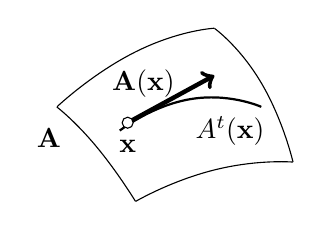
\begin{tikzpicture}
        % parallelogram
        \draw [] plot [smooth, tension=1]
        coordinates{(1, 0) (2, 0.4) (3, 0.5)};
        \draw [] plot [smooth, tension=1]
          coordinates{(3, 0.5) (2.6, 1.5) (2, 2.2)};
        \draw [] plot [smooth, tension=1]
          coordinates{(2, 2.2) (1, 1.9) (0, 1.2)};
        \draw [] plot [smooth, tension=1]
          coordinates{(0, 1.2) (0.5, 0.7) (1, 0)};

        % A
        \node [] at (-0.1, 0.8) {$\mathbf A$};

        % x
        \node [] at (0.9, 0.7) {$\mathbf x$};

        % A^t(x)
        \node [] at (2.2, 0.9) {$A^t(\mathbf x)$};

        % A(x)
        \node [] at (1.1, 1.5) {$\mathbf{ A(x)}$};
        % the curve A^t(x)
        \draw [thick] plot [smooth, tension=1]
          coordinates{(0.8, 0.9) (1.7, 1.3) (2.6, 1.2)};

        % the tangent vector
        \draw [ultra thick, ->] (0.9, 1.0) -- (2.0, 1.6);

        \draw [fill=white] (0.9, 1.0) circle (0.07);

      \end{tikzpicture}
      \label{fig:flow_vecfield}
      \caption{The group of diffeomorphism given by
      a vector field}
    \end{figure}

  \item
    The first-order differential operator $L_\mathbf{A}$.
    We refer here to the differentiation of functions
    in the direction of the field $\mathbf A$:
    for any function $\varphi: M \rightarrow \mathbb F$,
    the \emph{derivative in the direction of $\mathbb A$}
    is a new function $L_{\mathbf A} \varphi$,
    whose value at a point $\mathbf x$ is
    $$
    (L_{\mathbf A}\varphi) (\mathbf x)
    =
    \frac{d}{dt}\bigg|_{t = 0} \varphi(A^t\mathbf x).
    $$

\end{enumerate}

\begin{prob*}
  Show that the operator $L_\mathbf{A}$ is linear:
  $$
  L_\mathbf{A}(\lambda_1 \varphi_1 + \lambda_2 \varphi_2)
  =
  \lambda_1 L_\mathbf{A}\varphi_1
  +
  \lambda_2 L_\mathbf{A}\varphi_2
  \qquad
  (\lambda_1, \lambda_2 \in \mathbb{R}).
  $$
  Also, prove the Leibniz's formula
  $
  L_\mathbf{A}(\varphi_1\varphi_2)
  = \varphi_1 L_\mathbf{A} \varphi_2 + \varphi_2 L_\mathbf{A} \varphi_1.
  $

  \answer{
    For the linearity:
    $$
    \begin{aligned}
    L_\mathbf{A}(\lambda_1 \varphi_1 + \lambda_2 \varphi_2)
    &=
    \frac{d}{dt}\bigg|_{t = 0}
    \left[
    \lambda_1 \varphi_1(A^t\mathbf x)
    +
    \lambda_2 \varphi_2(A^t\mathbf x)
    \right]
    \\
    &=
    \lambda_1
    \frac{d}{dt}\bigg|_{t = 0}
    \varphi_1(A^t\mathbf x)
    +
    \lambda_2
    \frac{d}{dt}\bigg|_{t = 0}
    \varphi_2(A^t\mathbf x) \\
    &=
    \lambda_1
    (L_{\mathbf A}\varphi_1) (\mathbf x)
    +
    \lambda_2
    (L_{\mathbf A}\varphi_2) (\mathbf x).
    \end{aligned}
    $$

    For the Leibniz's formula:
    $$
    \begin{aligned}
    L_\mathbf{A}(\varphi_1 \varphi_2)
    &=
    \frac{d}{dt}\bigg|_{t = 0}
    \varphi_1(A^t\mathbf x)
    \varphi_2(A^t\mathbf x)
    \\
    &=
    \varphi_1(\mathbf x)
    \frac{d}{dt}\bigg|_{t = 0}
    \varphi_2(A^t\mathbf x)
    +
    \varphi_2(\mathbf x)
    \frac{d}{dt}\bigg|_{t = 0}
    \varphi_1(A^t\mathbf x) \\
    &=
    \varphi_1(\mathbf x)
    (L_{\mathbf A}\varphi_2) (\mathbf x)
    +
    \varphi_2(\mathbf x)
    (L_{\mathbf A}\varphi_1) (\mathbf x).
    \end{aligned}
    $$
  }
\end{prob*}

\begin{ex*}
  Let $(x_1, \dots, x_n$ be local coordinates on $M$.
  In this coordinate system the vector $\mathbf{ A(x) }$
  is given by its components
  $(A_1(\mathbf x), \dots, A_n(\mathbf x))$;
  the flow $A^t$ is given by the system of differential equations
  $$
  \dot x_1 = A_1(\mathbf x), \dots
  \dot x_n = A_n(\mathbf x)
  $$
  and, therefore, the derivative of
  $\varphi = \varphi(x_1, \dots, x_n)$
  in the direction $\mathbf A$ is
  $$
  L_\mathbf{A} \varphi = A_1 \frac{\partial \varphi}{\partial x_1}
  + \dots A_n \frac{ \partial \varphi }{ \partial x_n }.
  $$
  We could say that in the coordinates $(x_1, \dots, x_n)$
  the operator $L_\mathbf{A}$ has the form
  $$
  L_\mathbf{A} = A_1 \frac{\partial }{\partial x_1}
  + \dots + A_n \frac{ \partial }{ \partial x_n}.
  $$
  This is the general form of a first-order linear differential operator
  on coordinate space.
\end{ex*}

\begin{prob*}
  Show that the correspondences between vector fields $\mathbf A$,
  flows $A^t$, and differentiations $L_\mathbf{A}$ are one-to-one.

  \answer{
    The correspondence between the vector field $\mathbf A$
    and the differentiations $L_\mathbf{A}$ are apparent
    from the above example.
    For $\mathbf A$ and the flow, we first note that
    by definition the vector field $\mathbf{ A(x)}$ is determined by the flow.
    Conversely, we can trace the flow
    by following the vector field $\mathbf{ A(x) }$,
    That is,
    for a sufficiently small $\Delta t$,
    the flow approximately satisfies the recurrence relation
    $$
    A^t(\mathbf x) \approx
    A^{t-\Delta t}(\mathbf x + \Delta t \mathbf{A(x)})
    =
    A^{t-\Delta t} (1 + \Delta t \mathbf{A})\mathbf x.
    $$
    Or,
    $$
    A^t(\mathbf x)
    =
    \lim_{n\rightarrow \infty}
    \left(1 + \frac{t}{n} \mathbf{A}\right)^{n} \mathbf x.
    =
    \exp(t\mathbf{A}) \, \mathbf x.
    $$
    which means the flow is completely determined by the vector field.
  }
\end{prob*}

% subsection C
\subsection{Poisson bracket of vector fields}

Suppose that we are given two vector fields
$\mathbf A$ and $\mathbf B$ on a manifold $M$.
The corresponding flows $A^t$ and $B^s$
do not, in general commute:
$A^t B^s \ne B^s A^t$
(Figure 169).

    \begin{figure}
      \centering
      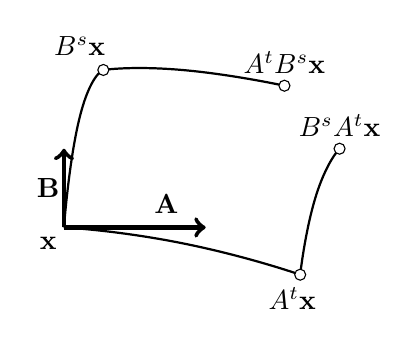
\begin{tikzpicture}
        % parallelogram
        \draw [thick] plot [smooth, tension=1]
          coordinates{(0, 0) (1.5, -0.2) (3, -0.6)};
          % A^t x
          \node [] at (2.9, -0.9) {$A^t \mathbf x$};

        \draw [thick] plot [smooth, tension=1]
          coordinates{(3, -0.6) (3.2, 0.4) (3.5, 1.0)};
          % B^s A^t x
          \node [] at (3.5,  1.3) {$B^s A^t \mathbf x$};

        \draw [thick] plot [smooth, tension=1]
          coordinates{(0.0, 0.0) (0.2, 1.4) (0.5, 2.0)};
          % B^s x
          \node [] at (0.2,  2.3) {$B^s \mathbf x$};

        \draw [thick] plot [smooth, tension=1]
          coordinates{(0.5, 2.0) (1.5, 2.0) (2.8, 1.8)};
          % A^t B^s x
          \node [] at (2.8,  2.1) {$A^t B^s \mathbf x$};

        \draw [fill=white] (3.0, -0.6) circle (0.07);
        \draw [fill=white] (3.5, 1.0) circle (0.07);
        \draw [fill=white] (0.5, 2.0) circle (0.07);
        \draw [fill=white] (2.8, 1.8) circle (0.07);

        % A
        \node [] at ( 1.3, 0.3) {$\mathbf A$};

        % B
        \node [] at (-0.2, 0.5) {$\mathbf B$};

        % x
        \node [] at (-0.2, -0.2) {$\mathbf x$};

        % the tangent vector
        \draw [ultra thick, ->] (0.0, 0.0) -- (1.8, 0.0);
        \draw [ultra thick, ->] (0.0, 0.0) -- (0.0, 1.0);

      \end{tikzpicture}
      \label{fig:noncommflows}
      \caption{Non-commutative flows}
    \end{figure}

\begin{prob*}
  Problem. Find an example.

  \solution{
    The fields $\mathbf A = \mathbf e_1$,
    $\mathbf B = x_1 \mathbf e_2$
    on the $(x_1, x_2)$ plane.

    \note{
      $$
      \begin{aligned}
        A^tB^s\mathbf x &= A^t (x_1, x_2 + x_1 s) = (x_1 + t, x_2 + x_1 s), \\
        B^sA^t\mathbf x &= B^s (x_1 + t, x_2) = (x_1 + t, x_2 + x_1 s + t s).
      \end{aligned}
      $$
    }
  }
\end{prob*}


To measure the degree of non-commutativity
of two flows $A^t$ and $B^s$ we consider the two points
$A^tB^s\mathbf x$ and $B^sA^t\mathbf x$.
%
In order to estimate the difference between these points,
we compare the value at them of some smooth function
$\varphi$ on the manifold $M$. The difference
$$
\Delta(t; s; \mathbf x)
=
\varphi(A^tB^s\mathbf x)
-
\varphi(B^sA^t\mathbf x)
$$
is clearly a differentiable function which is zero for $s = 0$
and for $t = 0$.
Therefore, the first term different from $0$ in the Taylor series
in $s$ and $t$ of $\Delta$ at $0$ contains $st$,
and the other terms of second order vanish.
%
We will calculate this principal bilinear term of $\Delta$ at $0$.

\note{
  At $t = 0$,
  $\Delta(0; s; \mathbf x) = \varphi(1 \, B^s \mathbf x) - \varphi(B^s \, 1 \mathbf x) = 0$.
  Similarly, for $s = 0$,
  $\Delta(t; 0; \mathbf x) = \varphi(A^t \, 1 \mathbf x) - \varphi(1 \, A^t \mathbf x) = 0$.
  So the Taylor series goes like
  $$
  \Delta(t; s; \mathbf x)
  = \Delta_{11} t s
  + \frac{\Delta_{12} }{1! \, 2!} t \, s^2
  + \frac{\Delta_{21} }{2! \, 1!} t^2 s + \dots
  $$
}

\begin{lem}
  The mixed partial derivative $\partial \Delta/\partial s \partial t$ at $0$
  is equal to the commutator of differentiation in the directions
  $\mathbf A$ and $\mathbf B$:
  $$
  \frac{\partial^2}{\partial s \partial t}\bigg|_{s=t=0}
  {\varphi(A^tB^s\mathbf x) - \varphi(B^sA^t\mathbf x)}
  =
  (L_\mathbf{B} L_\mathbf{A} \varphi
  -L_\mathbf{A} L_\mathbf{B} \varphi)
  (\mathbf x).
  $$
\end{lem}

\begin{proof}
  By the definition of $L_\mathbf{A}$,
  $$
  \frac{\partial}{\partial t}\bigg|_{t=0}
  \varphi(A^tB^s\mathbf x)
  =
  (L_\mathbf{A} \varphi)(B^s\mathbf x).
  $$
  If we denote the function $L_\mathbf{A}\varphi$ by $\psi$,
  then by the definition of $L_\mathbf{B}$
  $$
  \frac{\partial}{\partial s}\bigg|_{s=0}
  \psi(B^s\mathbf x)
  =
  (L_\mathbf{B} \psi)(\mathbf x).
  $$
  Thus,
  $$
  \frac{\partial^2}{\partial s \partial t}\bigg|_{s=t=0}
  \varphi(A^tB^s\mathbf x)
  =
  (L_\mathbf{B} L_\mathbf{A} \varphi)(\mathbf x).
  $$
\end{proof}

We now consider the commutator of differentiation operator
$L_\mathbf{B} L_\mathbf{A} - L_\mathbf{A} L_\mathbf{B}$.
%
At first glance this is a \emph{second}-order differential operator.

\begin{lem}
  The operator
  $L_\mathbf{B} L_\mathbf{A} \varphi-L_\mathbf{A} L_\mathbf{B} \varphi$
  is a first-order linear differential operator.
\end{lem}

\begin{proof}
  Let $(A_1, \dots, A_n)$ and $(B_1, \dots, B_n)$
  be the components of the fields $\mathbf A$ and $\mathbf B$
  in the local coordinate system $(x_1, \dots, x_n)$ on $M$.
  Then
  $$
  L_\mathbf{B} L_\mathbf{A} \varphi
  =
  \sum_{i=1}^n B_i \frac{\partial}{\partial x_i}
  \sum_{j=1}^n A_j \frac{\partial}{\partial x_j} \varphi
  =
  \sum_{i,j=1}^n
    B_i \frac{\partial A_j}{\partial x_i}
    \frac{\partial}{\partial x_j} \varphi
  +
  \sum_{i,j=1}^n
    B_i A_j
    \frac{\partial^2 \varphi}{\partial x_i \partial x_j} \varphi.
  $$
  If we subtract $L_\mathbf{A} L_\mathbf{B} \varphi$,
  the term with the second derivatives of $\varphi$ vanishes,
  and we obtain
  $$
  (L_\mathbf{B} L_\mathbf{A} - L_\mathbf{A} L_\mathbf{B}) \varphi
  =
  \sum_{i,j=1}^n
    \left(
      B_i \frac{\partial A_j}{\partial x_i}
      -
      A_i \frac{\partial B_j}{\partial x_i}
    \right)
    \frac{\partial}{\partial x_j} \varphi.
  $$
\end{proof}

\note{Notice the change of order of $A$ and $B$
  from $A^t B^s$ to $L_{\mathbf B}L_{\mathbf A}$.
  Example.
  In $\mathbb R^n$,
  for $B^s \mathbf x = e^s \mathbf x$,
  $$
  \frac{\partial}{\partial s}\bigg|_{s=0}
  \psi(e^s\mathbf x)
  =
  \sum_{i = 1}^n x_i \frac{ \partial \psi }{ \partial x_i }.
  $$
  So $L_\mathbf{B} = \mathbf x \cdot \nabla$,
  and $e^{s L_\mathbf{B}} \psi(\mathbf x) = \psi(e^s \mathbf x)$.
  %
  For $A^t \mathbf x = \mathbf x + t\mathbf a$,
  $$
  \frac{\partial}{\partial t}\bigg|_{t=0}
  \varphi(\mathbf x + t \mathbf a)
  =
  \sum_{i = 1}^n a_i \frac{ \partial \varphi }{ \partial x_i }.
  $$
  So $L_\mathbf{A} = \mathbf a \cdot \nabla$,
  and $e^{t L_\mathbf{A}} \varphi(\mathbf x) = \varphi(\mathbf x + t \mathbf a)$.
  Thus
  $$
  e^{s L_\mathbf{B}} e^{t L_\mathbf{A}} \varphi(\mathbf x)
  =
  e^{s L_\mathbf{B}} \varphi(\mathbf x + t\mathbf a)
  =
  \varphi(e^s \mathbf x + t\mathbf a).
  $$
  which corresponds to
  $A^t B^s \mathbf x = A^t (e^s \mathbf x) = e^s \mathbf x + t \mathbf a$.
  However,
  $$
  e^{t L_\mathbf{A}} e^{s L_\mathbf{B}} \varphi(\mathbf x)
  =
  e^{t L_\mathbf{A}} \varphi(e^s \mathbf x)
  =
  \varphi(e^s (\mathbf x + t\mathbf a) )
  $$
  does not.
  The point is that
  the first (innermost) operator applied to the coordinates $B^s$  
  corresponds to the last (outermost) differential operator
  applied to the function $e^{s L_\mathbf{B}}$.
  %
  For a chain of opertions,
  $\mathbf x \rightarrow B^s \mathbf x \rightarrow A^t B^s \mathbf x$,
  a flow operator, such as $A^t$ or $B^s$,
  applies on the current argument, or the current coordinates,
  so the first geometric operation
  goes into the innermost level.
  %
  On the other hand,
  differential operators for functions,
  like $e^{s L_\mathbf{B}}$ and $e^{t L_\mathbf{A}}$, always operate
  on $\mathbf x$ (instead of the argument of the function),
  so the operator corresponds to the first operation
  needs to be placed outermost to access
  the original $\mathbf x$.
}

Since every first-order linear differential operator is given by
a vector field, our operator
$L_\mathbf{B} L_\mathbf{A} - L_\mathbf{A} L_\mathbf{B}$
also corresponds to some vector field $L_\mathbf{C}$.


\begin{defn*}
  The \emph{Poisson bracket} or \emph{commutator}
  of two vector fields $\mathbf A$ and $\mathbf B$
  on a manifold $M$\footnote{In many books the bracket
    is given the opposite sign.
    Our sign agrees with  the sign of the commutator
    in the theory of Lie groups (cf. subsection F).}
  is the vector field $\mathbf C$, for which
  $$
  L_\mathbf{C} = L_\mathbf{B} L_\mathbf{A} - L_\mathbf{A} L_\mathbf{B}.
  $$
  The Poisson bracket of two vector fields is denoted by
  $\mathbf C = [ \mathbf A, \mathbf B ]$.
\end{defn*}

\begin{prob*}
  Suppose that the vector fields $\mathbf A$ and $\mathbf B$
  are given by their components $A_i$, $B_i$ in coordinates $x_i$.
  Find the components of the Poisson bracket.

  \solution{
    In the proof of Lemma 2, we proved the formula
    $$
    [\mathbf A, \mathbf B]_j =
    \sum_{i = 1}^n
      B_i \frac{ \partial A_j }{ \partial x_i }
      -
      A_i \frac{ \partial B_j }{ \partial x_i }.
    $$
  }
\end{prob*}


\begin{prob*}
  Let $\mathbf A_1$ be the linear vector field of velocities of a rigid body
  rotating with angular velocity $\pmb\omega_1$ around $\mathbf 0$,
  and $\mathbf A_2$ the same thing with $\pmb\omega_2$.
  Find the Poisson bracket $[\mathbf A_1, \mathbf A_2]$.

  \answer{Assuming summation over repeated indices.
    $A_{1j} = \epsilon_{jmn}\omega_{1m}x_n$,
    $\frac{ \partial A_{1j} }{ x_i } = \epsilon_{jmi}\omega_{1m}$,
    So
    $$
    \begin{aligned}
      A_{2i} \frac{ \partial A_{1j} }{ x_i }
      &= \epsilon_{ipq} \omega_{2p} x_q \epsilon_{jmi}\omega_{1m}
      = (\delta_{pj}\delta_{qm} - \delta_{pm}\delta_{qj}) \, \omega_{2p} x_q \omega_{1m} \\
      &= (\omega_{1m} x_m) \, \omega_{2j} - (\omega_{1m} \omega_{2m}) \, x_j.
    \end{aligned}
    $$
    By symmetry,
    $$
      A_{1i} \frac{ \partial A_{2j} }{ x_i }
      =
      (\omega_{2m} x_m) \, \omega_{1j} - (\omega_{1m} \omega_{2m}) x_j.
    $$
    Thus
    $$
    \begin{aligned}
      A_{2i} \frac{ \partial A_{1j} }{ x_i }
      -
      A_{1i} \frac{ \partial A_{2j} }{ x_i }
      &=
      (\omega_{1m} x_m) \, \omega_{1j}
      -
      (\omega_{2m} x_m) \, \omega_{1j} \\
      &=
      (\delta_{rm} \delta_{sj} - \delta_{sm} \delta_{rj} ) \omega_{1r} \omega_{2s} x_m
      \\
      &=
      \epsilon_{irs} \epsilon_{imj} \omega_{1r} \omega_{2s} x_m
      = [(\pmb\omega_1 \times \pmb\omega_2) \times \mathbf x]_j.
    \end{aligned}
    $$
    This shows the Poisson bracket represents a rotation with angular velocity
    $\pmb\omega_1 \times \pmb\omega_2$
    (and the author's choice of the sign of Poisson bracket
    is the natural one).
  }
\end{prob*}

% subsection 39D
\subsection{The Jacobi identity}

\begin{thm*}
  The Poisson bracket  makes the vector space of vector fields on a manifold $M$
  into a Lie algebra.
\end{thm*}

\begin{proof}
  Linearity and skew-symmetry of the Poisson bracket are clear.
  We will prove the Jacobi identity. By the definition of Poisson bracket,
  we have
  $$
  L_\mathbf{ [[A, B], C]} =
  L_{\mathbf C} L_\mathbf{ [A, B] } -L_\mathbf{ [A, B]} L_{\mathbf C}
  =
   L_{\mathbf C} L_{\mathbf B} L_{\mathbf A}
  -L_{\mathbf C} L_{\mathbf A} L_{\mathbf B}
  -L_{\mathbf B} L_{\mathbf A} L_{\mathbf C}
  +L_{\mathbf A} L_{\mathbf B} L_{\mathbf C}
  $$
  There will be 12 terms in all in the sum
  $ L_{\mathbf [[A, B], C]} + L_{\mathbf [[B, C], A]} + L_{\mathbf [[C, A], B]}$.
  Each term appears in the sum twice with opposite signs.
  \note{The other 8 terms:
  $$
  \begin{aligned}
  L_\mathbf{ [[B, C], A]}
  &=
  L_{\mathbf A} L_\mathbf{ [B, C] } -L_\mathbf{ [B, C]} L_{\mathbf A}
  =
   L_{\mathbf A} L_{\mathbf C} L_{\mathbf B}
  -L_{\mathbf A} L_{\mathbf B} L_{\mathbf C}
  -L_{\mathbf C} L_{\mathbf B} L_{\mathbf A}
  +L_{\mathbf B} L_{\mathbf C} L_{\mathbf A},  \\
  L_\mathbf{ [[C, A], B]}
  &=
  L_{\mathbf B} L_\mathbf{ [C, A] } -L_\mathbf{ [C, A]} L_{\mathbf B}
  =
   L_{\mathbf B} L_{\mathbf A} L_{\mathbf C}
  -L_{\mathbf B} L_{\mathbf C} L_{\mathbf A}
  -L_{\mathbf A} L_{\mathbf C} L_{\mathbf B}
  +L_{\mathbf C} L_{\mathbf A} L_{\mathbf B}.
  \end{aligned}
  $$
  }
\end{proof}

% subsection 39E
\subsection{A condition for the commutativity flows}

Let $\mathbf{A}$ and $\mathbf{B}$ be vector fields
on a manifold $M$.

\begin{thm*}
  The two flows $A^t$ and $B^s$ commute if and only if
  the Poisson bracket of the corresponding vectors fields
  $[\mathbf A, \mathbf B]$ is equal to zero.
\end{thm*}

% continue from clip 18


\summary{
  \begin{enumerate}
    \item A \emph{Lie algebra} is a vector space $L$ equipped with a
      \emph{Poisson bracket}, or \emph{commutator}, $[A, B]$,
      which is bilinear and satisfies the Jacobi identity:
      $$
      [[A, B], C] + [[B, C], A] + [[C, A], B] = 0.
      $$
      The Poisson bracket can be thought as a generalization
      of the vector product in three-dimensional space.

    \item Particularly, we studied the Lie algebra of vector fields
        $\mathbf A(\mathbf x)$.
        Each vector fields corresponds to a flow $A^t$
        and a Lie derivative
        $L_{\mathbf A} = \mathbf A \cdot \nabla
        = \sum_i A_i \frac{ \partial } { \partial x_i } $,
        which is a linear differential operator.

    \item The Poisson bracket $[\mathbf A, \mathbf B]$
        of two vector fields $\mathbf A$ and $\mathbf B$
        is defined through the Lie deriviative, such that
        $$
        L_\mathbf{[A, B]} = L_\mathbf{B} L_\mathbf{A} - L_\mathbf{A} L_\mathbf{B}.
        $$
        In components,
        $$
        [A, B]_j
        = \sum_i \left(
          B_i \frac{\partial A_j } { \partial x_i}
        - A_i \frac{\partial B_j } { \partial x_i}
          \right).
        $$
        (Remember the opposite sign, for Lie derivatives
        apply to functions, instead of points on the manifold.)

    \item The above Poisson bracket satisfies the Jacobi identity.
  \end{enumerate}
}



% section 40
\section{The Lie algebra of hamiltonian functions}

The hamiltonian vector fields on a symplectic manifold
form a subalgebra of the Lie algebra of all fields.
%
The hamiltonian functions also form a Lie algebra:
the operation in this algebra is called the Poisson bracket
of functions.
\note{The hamiltonian functions
also form a vector space.}
%
The first integrals of a hamiltonian phase flow form
a subalgebra of the Lie algebra of hamiltonian functions.


\begin{figure}[h]
  \centering
  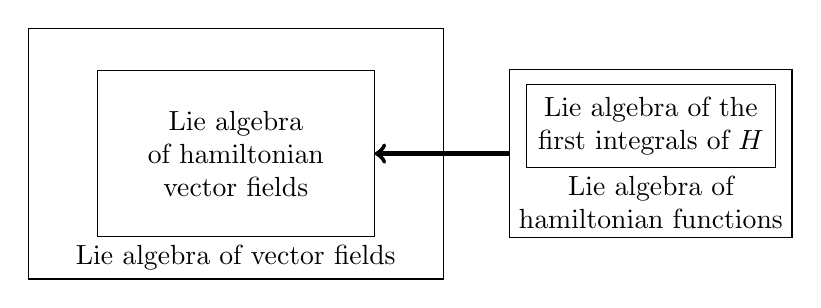
\begin{tikzpicture}
    \node (vf) at (0, 0)
      [draw, align=center, minimum size=9em, minimum width=15em]
      { \\[7em] Lie algebra of vector fields};
    \node (hamiltonianvf) at (0, 0)
      [draw, align=center, minimum size=6em, minimum width=10em]
      { Lie algebra \\ of hamiltonian \\ vector fields};

    \node (hamiltonianfunc) at (15em, 0)
      [draw, align=center, minimum size=6em, minimum width=10em]
      { \\[3em] Lie algebra of \\ hamiltonian functions}
      edge[ultra thick, ->] (hamiltonianvf);

    \node (firstintegrals) at (15em, 1em)
      [draw, align=center, minimum size=3em, minimum width=9em]
      { Lie algebra of the \\ first integrals of $H$ };
  \end{tikzpicture}
\end{figure}

% subsection 40A
\subsection{The Poisson bracket of two functions}

Let $(M^{2n}, \omega^2)$ be a symplectic manifold.
To a given function $H: M^{2n} \rightarrow \mathbb R$
on the symplectic manifold
there corresponds to a one-parameter
$g_H^t: M^{2n} \rightarrow M^{2n}$
of canonical transformations of $M^{2n}$--the
phase flow of the hamiltonian function equal to $H$.
%
Let $F: M^{2n} \rightarrow \mathbb R$
be another function on $M^{2n}$.

\begin{defn*}
  The \emph{Poisson bracket} $(F, H)$ of functions $F$ and $H$
  given on a symplectic manifold $(M^{2n}, \omega^2)$
  is the derivative of the function $F$ in the direction of
  the phase flow with hamiltonian function $H$:
  $$
  (F, H)(\mathbf x)
  =
  \left. \frac{ d }{ dt } \right|_{t = 0}
  F( g_H^t( \mathbf x ) ).
  $$
  Thus, the Poisson bracket of two functions on $M$ is again
  a function on $M$.
\end{defn*}

% Corollary 1
\begin{cor}
  A function $F$ is a first integral of the phase flow
  with hamiltonian function $H$ if and only if its Poisson bracket
  with $H$ is identically zero: $(F, H) \equiv 0$.
\end{cor}

We can give the definition of Poisson bracket in a slightly
different from if we use the isomorphism $I$ between 1-forms
and vector fields on a symplectic manifold $(M^{2n}, \omega^2)$.
%
%\note{Cf. Sec. 39C. The 1-form $\omega^1$ is mapped to $I\omega^1$
%such that $\omega^1(\pmb\eta) \equiv \omega^2(\pmb\eta, I\omega^1)$.
%}
%
This isomorphism is defined by the relation (cf. Section 37)
$$
\omega^2(\pmb\eta, I\omega^1)
=
\omega^1(\pmb\eta).
$$
The velocity vector of the phase flow $g_H^t$ is $IdH$.
This implies
(\note{$\omega^1 = dF$, $\pmb\eta = IdH$.})

% Corollary 2
\begin{cor}
  The Poisson bracket of the functions $F$ and $H$
  is equal to the value of the 1-form $dF$
  on the velocity vector $IdH$ of the phase flow with
  hamiltonian function $H$:
  $$
  (F, H) = dF(IdH).
  $$
\end{cor}

Using the preceding formula again, we obtain

% Corollary 3
\begin{cor}
  The Poisson bracket of the functions $F$ and $H$ is equal to the
  ``skew scalar product'' of the velocity vectors of the phase flows
  with hamiltonian functions $H$ and $F$:
  $$
  (F, H) = \omega^2(IdH, IdF).
  $$
\end{cor}

It is now clear that

% Corollary 4
\begin{cor}
  The Poisson bracket of the functions $F$ and $H$
  is a skew-symmetric bilinear function of $F$ and $H$:
  $$
  (F, H) = -(H, F)
  $$
  and
  $$
  (H, \lambda_1 F_1 + \lambda_2 F_2)
  =
  \lambda_1 (H, F_1)
  +
  \lambda_2 (H, F_2)
  \qquad
  (\lambda_1 \in \mathbb R).
  $$
\end{cor}

Although the above arguments are obvious,
they lead to nontrivial deductions,
including the following generalization
of a theorem of E. Noether.

\begin{thm*}
  If a hamiltonian function $H$ on a symplectic manifold $(M^{2n}, \omega^2)$
  admits the one-parameter group of canonical transformations
  given by a hamiltonian $F$,
  then $F$ is a first integral of the system with hamiltonian function $H$.
\end{thm*}

\begin{proof}
  Since $H$ is a first integral of the flow $g_F^t$,
  $(H, F) = 0$ (Corollary 1).
  Therefore $(F, H) = 0$ (Corollary 4)
  and $F$ is a first integral (Corollary 1).

  \note{
    $(F, H) = \left.\frac{d}{dt}\right|_{t = 0}F(g_H^t(\mathbf x)) = 0$.
  }
\end{proof}

% Problem 1
\begin{prob}
  Compute the Poisson bracket of two functions $F$ and $H$
  in the canonical coordinates
  $\mathbb R^{2n} = \{(\mathbf p, \mathbf q)\}$,
  $\omega^2(\pmb\xi, \pmb\eta) = (I\pmb\xi, \pmb\eta)$.
  \note{The last formula is only true in
  the canonical coordinates.
  Cf. the note in subsection 37C.}

  \solution{
    By the Corollary 3 we have
    $$
    (F, H) =
    \sum_{i = 1}^n
      \frac{ \partial H } { \partial p_i } \frac{ \partial F } { \partial q_i }
      -
      \frac{ \partial H } { \partial q_i } \frac{ \partial F } { \partial p_i }
    $$
    (we use the fact that $I$ is symplectic and has the form
    $$
    I = \left(\begin{array}{ccc}
        0 & -E \\
        E & 0
    \end{array}\right)
    $$
    in the basis $(\mathbf p, \mathbf q)$).
  }
\end{prob}

% Problem 2
\begin{prob}
  Compute the Poisson brackets of the basic functions $p_i$ and $q_i$.

  \solution{
    The gradients of the basic functions form a ``symplectic basis'':
    their skew-scalar products are
    $$
    (p_i, p_j) = (p_i, q_j) = (q_i, q_j) = 0 \quad (\mathrm{if}\; i\ne j)
    \qquad
    (q_i, p_i) = -(p_i, q_i) = 1.
    $$
  }
\end{prob}

% Problem 3
\begin{prob}
  Show that the map $A: \mathbb R^{2n} \rightarrow R^{2n}$
  sending $(\mathbf p, \mathbf q) \rightarrow
  (\mathbf P(\mathbf p, \mathbf q), \mathbf Q(\mathbf p, \mathbf q))$
  is canonical if and only if the Poisson brackets of any two
  functions in the variables $(\mathbf p, \mathbf q)$
  and $(\mathbf P, \mathbf Q)$ coincide:
  $$
  (F, H)_\mathbf{p, q}
  =
  \frac{\partial H}{\partial \mathbf p} \frac{\partial F}{\partial \mathbf q}
  -
  \frac{\partial H}{\partial \mathbf q} \frac{\partial F}{\partial \mathbf p}
  =
  \frac{\partial H}{\partial \mathbf P} \frac{\partial F}{\partial \mathbf Q}
  -
  \frac{\partial H}{\partial \mathbf Q} \frac{\partial F}{\partial \mathbf P}
  =
  (F, H)_\mathbf{P, Q}.
  $$

  \solution{
    \note{The ``only if'' part: canonical $\rightarrow$ Poisson brackets coincide.}
    Let $A$ be canonical.
    %
    Then the symplectic structure $d\mathbf p \wedge d\mathbf q$
    and $d\mathbf P \wedge d\mathbf Q$ coincide.
    \note{This is equivalent to saying $\int_c \omega^2 = \int_{gc} \omega^2$.}
    But the definition of the Poisson bracket $(F, H)$
    was given invariably in terms of the symplectic structure;
    it did not involve the coordinates. Therefore,
    $$
    (F, H)_\mathbf{p, q} = (F, H) = (F, H)_\mathbf{P, Q}.
    $$
    \note{The ``if'' part: Poisson brackets coincide $\rightarrow$ canonical.}
    Conversely, suppose that the Poisson brackets
    $(P_i, Q_j)_\mathbf{p, q}$ have the standard form
    of Problem 2.
    Then, clearly $d\mathbf P \wedge d\mathbf Q = d\mathbf p \wedge d\mathbf q$,
    i.e., the map is canonical.

    \note{
      Alternative argument for the ``if'' part:
      if $(F, H)_\mathbf{p, q} = (F, H)_\mathbf{P, Q}$ for $\forall F, H$,
      then $d\mathbf p \wedge d\mathbf q = d\mathbf P \wedge d\mathbf Q$.

      Let $\mathbf x = (\mathbf p, \mathbf q)$,
      $\mathbf X = (\mathbf P, \mathbf Q)$,
      we have
      $$
      \begin{aligned}
      (F, H)_\mathbf{p, q}
      &=
      \sum_{k,l} J^{kl}
        \frac{ \partial F } { \partial x^k }
        \frac{ \partial H } { \partial x^l }
      =
      \sum_{k,l,K,L} J^{kl}
        \frac{ \partial F } { \partial X^K }
        \frac{ \partial X^K } { \partial x^k }
        \frac{ \partial H } { \partial X^L }
        \frac{ \partial X^L } { \partial x^l }
      \\
      (F, H)_\mathbf{P, Q}
      &=
      \sum_{K,L} J^{KL}
        \frac{ \partial F } { \partial X^K }
        \frac{ \partial H } { \partial X^L }.
      \end{aligned}
      $$
      Since the two expression are supposed to be the same,
      we conclude
      \begin{equation}
      \sum_{k,l} J^{kl}
        \frac{ \partial X^K } { \partial x^k }
        \frac{ \partial X^L } { \partial x^l }
      = J^{KL}.
      \label{eq:symplectic_condition}
      \end{equation}

      Now let us expand the 2-form $\omega^2(\pmb\xi,\pmb\eta)$
      in components.
      First we shall review the meaning of ``components'' $\xi_k$ of a vector $\pmb\xi$.
      For a scalar $\phi$, we have
      $$
      d\phi = \sum_k \frac{ \partial \phi } { \partial x^k } dx^k
      \qquad \mathrm{and} \qquad
      d\phi
      = \sum_K \frac{ \partial \phi } { \partial X^K } dX^K
      = \sum_{k, K} \frac{ \partial \phi } { \partial X^K }
      \frac{ \partial X^K } { \partial x^k } d x^k.
      $$
      So
      $$
      \frac{ \partial \phi } { \partial x^k }
      =
      \sum_K \frac{ \partial \phi } { \partial X^K } \frac { \partial X^K } { \partial x^k },
      $$
      The components $\xi_k$ of a (covariant) vector $\pmb\xi$ are quantities
      behaves like $\partial \phi/\partial x^k$.  So
      %
      $$
      \xi_k = \sum_K \xi_K \frac { \partial X^K } { \partial x^k }.
      $$

      Now for the 2-form
      $$
      \begin{aligned}
      \omega^2(\pmb\xi, \pmb\eta)
      &=
      \sum_{k,l} J^{kl} \xi_k \eta_l
      =
      \sum_{k,l,K,L} J^{kl} \frac{ \partial X^K } { \partial x^k }
        \frac{ \partial X^L } { \partial x^l } \xi_K \xi_L \\
      &\stackrel{\eqref{eq:symplectic_condition}}{=\joinrel=}
      \sum_{K,L} J^{KL} \xi_K \xi_L.
      \end{aligned}
      $$
      The last expression is $\omega^2(\pmb\xi, \pmb\eta)$
      written in coordinates $\mathbf X = (\mathbf P, \mathbf Q)$.
      So this is precisely the statement
      $d\mathbf p \wedge d\mathbf q = d\mathbf P \wedge d\mathbf Q$
      in component form.
    }
  }
\end{prob}

% Problem 4
\begin{prob}
  Show that the Poisson bracket of a product can be calculated by Leibniz's rule:
  $$
  (F_1 F_2, H) = F_1 (F_2, H) + F_2 (F_1, H).
  $$

  \hint{The Poisson bracket $(F_1 F_2, H)$ is the derivative of the product $F_1 F_2$
  in the direction of the field $IdH$.}

  \answer{
    $$(F_1 F_2, H) = d(F_1 F_2)(IdH) = F_1 dF_2(IdH) + F_2 dF_1(IdH)
    = F_1(F_2, H) + F_2 (F_1, H).$$
  }
\end{prob}






\begin{figure}[h]
  \centering
 \begin{tikzpicture}
    \draw (-1,0) to[bend left] (1,0);
    \draw (-1.2,.1) to[bend right] (1.2,.1);
    \draw[rotate=0] (0,0) ellipse (100pt and 50pt);
  \end{tikzpicture}
\end{figure}



\section{Symplectic geometry}

\section{Parametric resonance in systems with many degrees of freedom}

\section{A symplectic atlas}

\chapter{Canonical formalism}

\section{The integral invariant of Poincar\'e-Cartan}

\section{Applications of the integral invariant of Poincar\'e-Cartan}

\section{Huygens' principle}

\section{The Hamilton-Jacobi method for integrating Hamilton's canonical equations}

\section{Generating functions}

\chapter{Introduction to perturbation theory}

\section{Integrable systems}

\section{Action-angle variables}

\section{Averaging}

\section{Averaging of perturbations}

\appendix
\renewcommand{\thechapter}{\arabic{chapter}}

\chapter{Riemannian curvature}

\chapter{Geodesics of left-invariant metrics on Lie groups and
the hydrodynamics of ideal fluids}

\chapter{Symplectic structures on algebraic manifolds}

\chapter{Contact structures}

\chapter{Dynamical systems with symmetries}

\chapter{Normal forms of quadratic hamiltonians}

\chapter{Normal forms of hamiltonian systems near stationary points
and closed trajectories}

\chapter{Theory of perturbations of conditionally periodic motion,
and Kolmogorov's theorem}

\chapter{Poincar\'e's geometric theorem, its generalizations and
applications}

\chapter{Multiplicities of characteristic frequencies, and ellipoids
depending on parameters}

\chapter{Short wave asymptotics}

\chapter{Lagrangian singularities}

\chapter{The Korteweg-de Vries equation}

\chapter{Poisson structures}

\chapter{On elliptic coordinates}

\chapter{Singularities of ray systems}

\end{document}
